%%=============================================================================
%% Methodologie
%%=============================================================================

\chapter{\IfLanguageName{dutch}{Methodologie}{Methodology}}%
\label{ch:methodologie}

%% TODO: In dit hoofstuk geef je een korte toelichting over hoe je te werk bent
%% gegaan. Verdeel je onderzoek in grote fasen, en licht in elke fase toe wat
%% de doelstelling was, welke deliverables daar uit gekomen zijn, en welke
%% onderzoeksmethoden je daarbij toegepast hebt. Verantwoord waarom je
%% op deze manier te werk gegaan bent.
%% 
%% Voorbeelden van zulke fasen zijn: literatuurstudie, opstellen van een
%% requirements-analyse, opstellen long-list (bij vergelijkende studie),
%% selectie van geschikte tools (bij vergelijkende studie, "short-list"),
%% opzetten testopstelling/PoC, uitvoeren testen en verzamelen
%% van resultaten, analyse van resultaten, ...
%%
%% !!!!! LET OP !!!!!
%%
%% Het is uitdrukkelijk NIET de bedoeling dat je het grootste deel van de corpus
%% van je bachelorproef in dit hoofstuk verwerkt! Dit hoofdstuk is eerder een
%% kort overzicht van je plan van aanpak.
%%
%% Maak voor elke fase (behalve het literatuuronderzoek) een NIEUW HOOFDSTUK aan
%% en geef het een gepaste titel.

Om de centrale onderzoeksvraag te beantwoorden: “Hoe kan men Suricata en Zeek als Intrusion Detection Systems (IDS) optimaliseren voor een gesimuleerde IoT omgeving in een klein bedrijf met nadruk op resourcegebruik (CPU/geheugen), vlotte schaalbaarheid en detectienauwkeurigheid?” werd gedurende dit project een gestructureerde, stapsgewijze aanpak gevolgd. 

\vspace{1em}
\textbf{Fase 1: Tools en netwerktopologie (Ontwerp)} \\
De eerste stap in het onderzoek richt zich op het ontwerpen van een netwerktopologie die een kmo-omgeving representatief simuleert. Binnen deze fase worden de rollen en verantwoordelijkheden van alle hardware- en softwarecomponenten gedefinieerd. Hierbij wordt vastgesteld hoe het netwerkverkeer passief zichtbaar kan worden gemaakt voor de detectiesystemen, en hoe fysieke ESP32-microcontrollers en Tuya-endpoints worden geconfigureerd om realistische IoT-telemetriedata te genereren.

\textbf{Verantwoording:} Het gebruik van fysieke hardware-endpoints in plaats van puur gesimuleerde netwerkstromen is noodzakelijk om de daadwerkelijke netwerkoverhead, inclusief natuurlijke pakketvertragingen (jitter en latency), realistisch in kaart te brengen.

\vspace{0.5cm}

\textbf{Fase 2: Installatie en configuratie (Implementatie)} \\
Zodra de fysieke netwerkinfrastructuur is ontworpen, verschuift de focus naar de softwarematige inrichting van de systemen. Deze fase omvat de gedetailleerde installatie en configuratie van Suricata en Zeek op de Raspberry Pi-sonde. Daarnaast wordt de configuratie van de centrale IoT-diensten gerealiseerd, waaronder de Eclipse Mosquitto MQTT-broker, de Zigbee2MQTT-gateway en het Home Assistant-platform.

\textbf{Verantwoording:} Door deze diensten lokaal en onafhankelijk van cloudverbindingen in te richten, wordt de netwerkomgeving representatief voor kmo's die hun datastromen om privacy- en veiligheidsredenen on-premise willen houden.

\vspace{0.5cm}

\textbf{Fase 3: Ontwikkeling van custom rules (Threat Engineering)} \\
Omdat standaardregels vaak ontoereikend zijn voor het detecteren van de specifieke communicatiepatronen van IoT-apparaten, richt deze fase zich op het schrijven van op maat gemaakte signature-regels voor Suricata en gedragsscripts voor Zeek.

\textbf{Verantwoording:} Het schrijven van custom rules is essentieel om alert fatigue (een overvloed aan valse meldingen) te voorkomen, wat een van de grootste operationele drempels is voor kmo's met beperkte IT-beheercapaciteit.

\vspace{0.5cm}

\textbf{Fase 4: Aanvalsscenario's en actieve validatie} \\
Om de effectiviteit en robuustheid van de geconfigureerde detectiesystemen in de praktijk te valideren, worden gecontroleerde penetratietests uitgevoerd. Er worden drie specifieke aanvalsscenario's getest: een Denial of Service (DoS/MQTT-flood), een onjuist opgebouwde of gemanipuleerde MQTT-payload, en een actieve poortscan.

\textbf{Verantwoording:} Actieve aanvalssimulaties zijn de enige methode om empirisch te bewijzen of de geconfigureerde NIDS in staat is om kwaadaardige activiteiten in realtime te onderscheiden van legitiem sensorverkeer.

\vspace{0.5cm}

\textbf{Fase 5: Verzamelen en analyseren van meetgegevens} \\
Tot slot is het essentieel om het resourcegebruik in kaart te brengen dat Suricata en Zeek genereren wanneer zij parallel als standalone IDS op een Raspberry Pi draaien. Het verbruik van systeembronnen (CPU-belasting, geheugenbeslag en eventueel pakketverlies) wordt structureel gemeten in drie verschillende netwerkstatussen:

\begin{itemize}
    \item \textbf{Rusttoestand (idle):} Wanneer er geen netwerkverkeer wordt gecapteerd.
    \item \textbf{Operationele toestand (baseline):} Tijdens de verwerking van regulier, legitiem IoT-verkeer.
    \item \textbf{Aanvalstoestand (stress-test):} Wanneer er actieve netwerkaanvallen op de infrastructuur worden uitgevoerd.
\end{itemize}

\textbf{Verantwoording:} Deze driedelige meting maakt het mogelijk om de exacte computationele kostprijs per detectiemethode te berekenen, wat direct bijdraagt aan de beantwoording van de hoofdonderzoeksvraag omtrent resource-optimalisatie.

\chapter{\IfLanguageName{dutch}{Tools en netwerktopologie}{Tools en netwerktopologie}}%
\label{ch:Tools en netwerktopologie}

Dit hoofdstuk vormt de eerste fase van de Proof of Concept (PoC). Om bruikbare en betrouwbare meetresultaten uit de testomgeving te verkrijgen, is er bewust gekozen voor het gebruik van refurbished hardwarecomponenten. Deze benadering sluit direct aan bij de budgettaire en operationele realiteit van kleine tot middelgrote ondernemingen (kmo's).


Om een dergelijke kmo accuraat na te bootsen werd er een netwerktopologie ontworpen waarin de MQTT-broker lokaal draait. Binnen dit hoofdstuk worden alle netwerkcomponenten, de virtualisatielaag, de IoT-eindpunten en de positionering van de Intrusie Detectie Systeem (IDS) gedetailleerd beschreven (zie Figuur \ref{fig:NetwerkTopologieIoT}).

 
\begin{figure}[H]
    \centering
    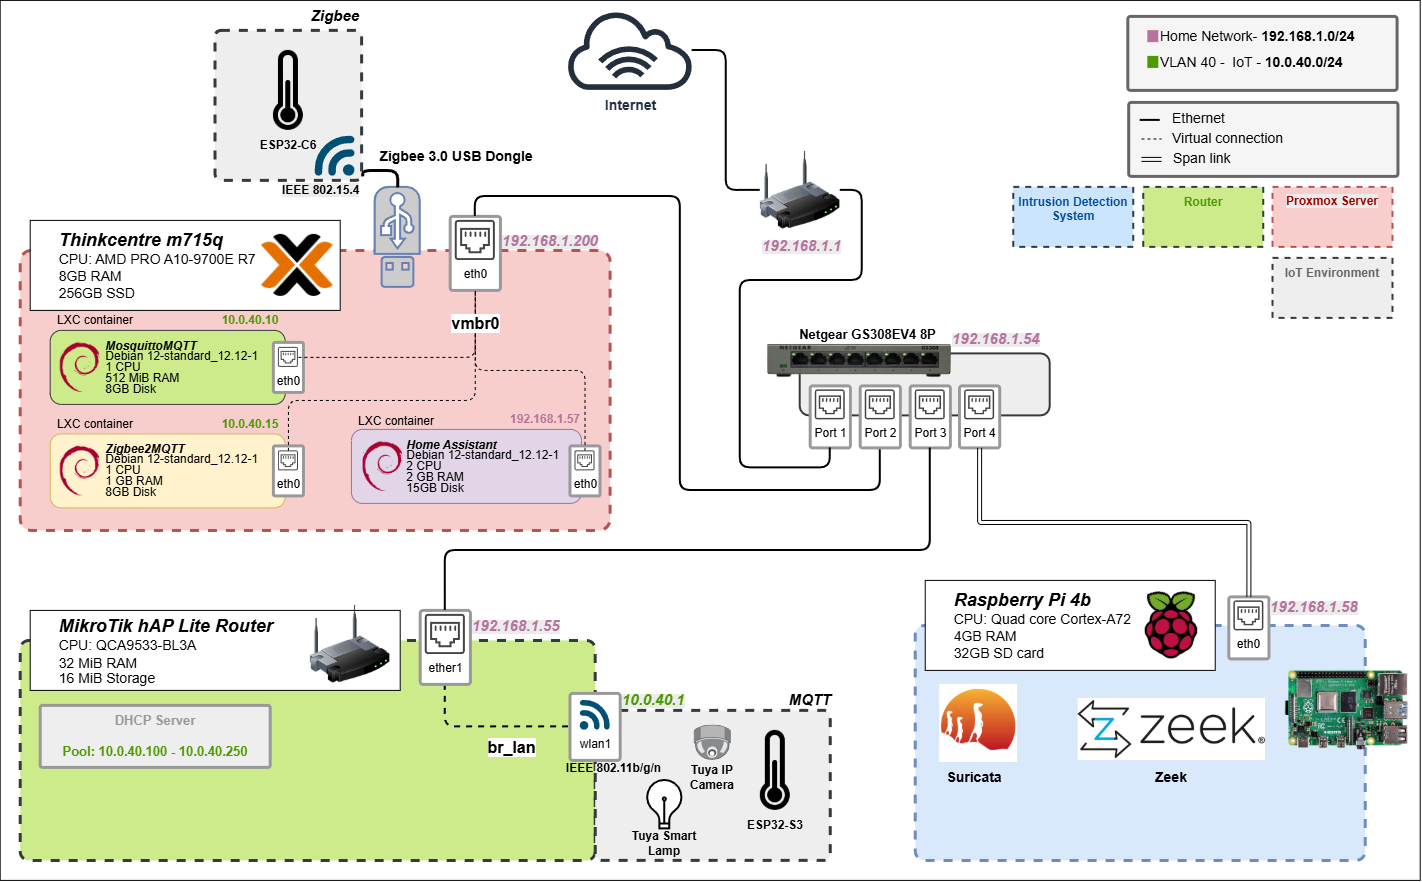
\includegraphics[width=1\textwidth]{../graphics/NetwerkTopologieIoT.png}
    \caption{ Logische netwerktopologie van de gesimuleerde kmo-testomgeving (Proef of Concept.)}
    \label{fig:NetwerkTopologieIoT}
\end{figure}

\section{Hardwarecomponenten}

In deze sectie worden de fysieke hardwarecomponenten beschreven die de onderliggende infrastructuur (de fysieke laag) van de Proof of Concept vormen. Om de neutraliteit, herbruikbaarheid en reproduceerbaarheid van het academische ontwerp te waarborgen, wordt elk fysiek apparaat gekarakteriseerd op basis van zijn functionele rol en logische positie binnen de topologie.
\vspace{1em}

\textbf{Server (ThinkCentre m715q)} \\
Deze refurbished server is uitgerust met een AMD Ryzen 5 Pro 2400GE-processor, 16 GB RAM en een 256 GB SSD. Het apparaat draait op Proxmox VE, een open-source virtualisatieplatform dat KVM-virtualisatie en LXC-containers ondersteunt.
Dit systeem fungeert als de onderliggende hypervisor waarop Proxmox VE draait. De primaire taak van deze hostomgeving is het simuleren van verschillende diensten die binnen LXC-containers (Linux Containers) draaien. Binnen deze architectuur host de server drie specifieke componenten:
\begin{itemize}
    \item \textbf{Eclipse Mosquitto MQTT:} Deze component fungeert als de lokale MQTT-broker binnen het netwerk.
    \item \textbf{Zigbee2MQTT:} Dit fungeert als de protocol-gateway. Deze dienst vertaalt de communicatie van Zigbee-apparaten naar IP-gebaseerde MQTT-berichten, zodat deze over het netwerk kunnen worden geanalyseerd.
    \item \textbf{Home Assistant:} Dit is het centrale beheerplatform waarop de verzamelde data visueel wordt weergegeven.
\end{itemize}
\vspace{1em}

\textbf{Switch (Netgear GS308EV4)} \\
Deze 8-poorts gigabit switch is een managed switch die ondersteuning biedt voor VLAN-configuraties. Binnen de netwerktopologie vormt deze fysieke switch het centrale knooppunt voor de aangesloten apparatuur. Aangezien het een managed switch betreft, kan een netwerkpoort worden geconfigureerd als een Switched Port Analyzer (SPAN) link. Hierdoor kan het inkomende en uitgaande netwerkverkeer op hardwareniveau worden gedupliceerd en ter inspectie direct worden doorgestuurd naar het NIDS.
\vspace{1em}


\textbf{Router (MikroTik hAP ac lite)} \\
Deze enterprise-grade router draait op RouterOS, een besturingssysteem dat een volledige en gedetailleerde configuratie van het netwerk ten behoeve van de IoT-apparaten mogelijk maakt. De primaire functie van deze component is netwerksegmentatie, waarbij het IoT-verkeer (VLAN 40) strikt wordt gescheiden van het reguliere netwerkverkeer. Door de isolatie van dit IoT-verkeer wordt een netwerkarchitectuur gerealiseerd waarin potentieel kwetsbare eindpunten binnen een gecontroleerde, gesloten zone opereren. Daarnaast fungeert het apparaat as de lokale DHCP-server voor de geëmuleerde testomgeving.
\vspace{1em}

\textbf{NIDS (Raspberry Pi 4 Model B)} \\
Voor de passieve beveiligingstelemetrie en anomaliedetectie is een Raspberry Pi 4 Model B ingezet als dedicated Network Intrusion Detection System (NIDS). Deze single-board computer draait op Raspberry Pi OS Lite (64-bit). De specifieke use case van dit toestel is het passief inspecteren en analyseren van het netwerkverkeer dat wordt doorgestuurd via de mirror-poort (SPAN) van de switch (Netgear GS308EV4). Op dit systeem zijn de open-source detectiesystemen Suricata en Zeek geïnstalleerd, maar deze opereren strikt gescheiden van elkaar. Om een objectieve vergelijkende analyse uit te kunnen voeren, is telkens slechts één IDS-engine actief.
\vspace{1em}

\textbf{IoT-eindpunten (ESP32 en Tuya-endpoints)} \\
De IoT-eindpunten bestaan uit een combinatie van fysieke ESP32-microcontrollers en Tuya-gebaseerde apparaten. De ESP32-microcontrollers zijn geprogrammeerd om realistische telemetriegegevens te genereren, terwijl de Tuya-endpoints standaard IoT-apparaten representeren.

\begin{itemize}
    \item \textbf{ESP32-microcontrollers:} Deze microcontrollers zijn geprogrammeerd om een reeks van sensordata te genereren, zoals temperatuur. 
    \begin{itemize}
        \item \textbf{ESP32-S3:} Genereert continu IP-gebaseerde telemetriedata vanuit het geïsoleerde VLAN 40, die via poort 1883 rechtstreeks naar de lokale Mosquitto MQTT-broker wordt gepubliceerd.
        \item \textbf{ESP32-C6:} Deze microcontroller is geconfigureerd om Zigbee-berichten te genereren, die vervolgens via de Zigbee2MQTT-gateway worden vertaald naar MQTT-berichten. Deze berichten worden eveneens gepubliceerd naar de lokale Mosquitto MQTT-broker.
    \end{itemize}
    \item \textbf{Tuya-endpoints:} Deze apparaten zijn standaard IoT-apparaten die communiceren via het Tuya-protocol. Ze dienen als representatieve voorbeelden van commerciële IoT-apparaten die in een kmo-omgeving kunnen worden ingezet.
\end{itemize}


\section{Softwareinstrumenten}
Naast de fysieke en virtuele hardwarecomponenten, omvat de testomgeving een reeks software-instrumenten die essentieel zijn voor het verzamelen, visualiseren en valideren van netwerkverkeer en telemetriegegevens.
\vspace{1em}

\textbf{tcpdump:} Dit command-line netwerkprotocol-analysetool wordt gebruikt om het netwerkverkeer te capteren en valideren van de SPAN-poort van de switch. Het biedt een gedetailleerde weergave van de netwerkpakketten, inclusief bron- en bestemmingsadressen, protocollen en payload-inhoud.

\vspace{1em}

\textbf{nmap:} Dit open-source netwerkverkenningstool wordt ingezet om een portscan scenario uit te voeren. Het genereert een reeks van netwerkverkeer dat door de NIDS moet worden gedetecteerd, waardoor de effectiviteit van de IDS-configuratie kan worden geëvalueerd.

\vspace{1em}

\textbf{Python(Scapy en Socket):} Voor het genereren van een Denial of Service (DoS) en het manipuleren van MQTT-payloads wordt Python gebruikt, met name de Scapy- en Socket-bibliotheken.

\vspace{1em}

\textbf{Python(Metrieken):} Voor het verzamelen van resourcegebruik (CPU, geheugen) van de NIDS wordt een Python-script gebruikt dat periodiek systeemstatistieken verzamelt en logt.

\vspace{1em}

\textbf{Tuyadeveloper platform:} Voor het vinden van de juiste Tuya-endpoints en het verkrijgen van de bijbehorende API-sleutels wordt het Tuyadeveloper platform gebruikt. 


\chapter{\IfLanguageName{dutch}{Installatie en configuratie}{Installatie en configuratie}}%
\label{ch:Installatie en configuratie}
\subsection{Proxmox nodes configuratie}
\vspace{1em}
\textbf{Mosquitto MQTT-broker Configuratie}


De Eclipse Mosquitto MQTT-broker is geïmplementeerd binnen de Proxmox server als een Linux Container (LXC). Om de virtuele infrastructuur efficiënt te benutten zijn de systeembronnen voor deze Debian-container bewust minimaal gehouden: één CPU-core, 512 MB ugen en 8 GB opslag. De virtuele netwerkinterface van deze containers is gekoppeld aan de virtuele Proxmox-bridge (\texttt{vmbr0}) en geconfigureerd met de vlan tag 40 (Zie Figuur \ref{fig:netwerk}). Dit zorgt ervoor dat al het netwerkverkeer de container strikt geïsoleerd blijft binnen het IoT-subnet.werkgehe

\begin{figure}[H]
    \centering
    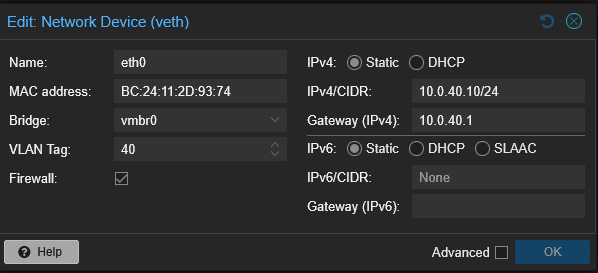
\includegraphics[width=0.7\textwidth]{../graphics/Proxmox/netConf.png}
    \caption{Virtuele netwerkconfiguratie van de Proxmox LXC-containers.}
    \label{fig:netwerk}
\end{figure}




\vspace{1em}
\textbf{Zigbee2MQTT Configuratie}


De Zigbee2MQTT-gateway is ook als een Linux Container geconfigureerd op de Proxmox server, waar deze als brug dient tussen het draadloze Zigbee-protocol en het IP-gebaseerde MQTT-netwerk. Omdat het netwerkverkeer continu vertaald moet worden, heeft deze LXC meer werkgeheugen (1024 MB) nodig. Wat netwerkisolatie betreft, volgt deze container dezelfde strikte ontwerpprincipes als de MQTT-broker. Aan deze container is een fysieke Zigbee USB-dongle verbonden die als Zigbee Coordinator (ZC) werkt. Zigbee End Devices (ZED), zoals de ESP32-C6, kunnen hiermee verbinden om telemetriedata door te sturen.

\vspace{1em}
\textbf{Home Assistant Configuratie}

Binnen het netwerk werkt Home Assistant als het centrale beheerplatform van de IoT-omgeving. Het doel van dit LXC is om de aangesloten IoT-toestellen, zoals de microcontrollers en Tuya-toestellen, te visualiseren en deze overzichtelijk op een dashboard weer te geven (zie Figuur. \ref{fig:HomeAssistantDash})

\begin{figure}[H]
    \centering
    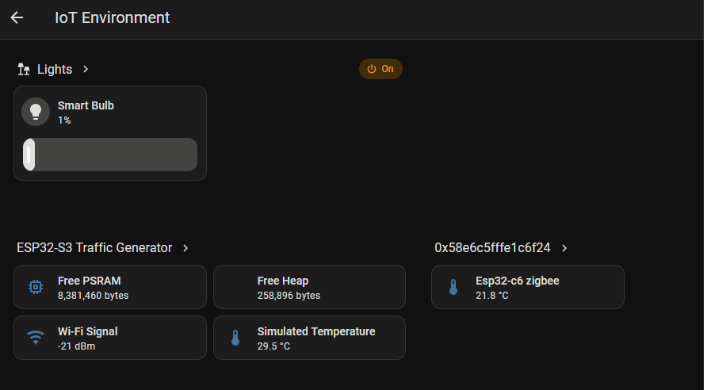
\includegraphics[width=0.7\textwidth]{../graphics/Proxmox/HomeAssistantDash.png}
    \caption{Home Assistant Dashboard.}
    \label{fig:HomeAssistantDash}
\end{figure}

\subsection{Raspberry Pi 4 Model B installatie en configuratie}

Voor een consistente analyse en evaluatie van de gekozen NIDS is er bewust gekozen om het besturingssysteem en beide monitoringtools op een enkele SD-kaart te installeren. Een belangrijke punt van deze configuratie is dat Suricata en Zeek nooit gelijktijdig draaien, dit zorgt ervoor dat beide systemen niet met elkaar moeten concurreren voor systeembronnen.

Als gekozen besturingssysteem werd er gekozen voor de Raspberry Pi OS Lite, zodat Suricata en Zeek tijdens de analysefase over meer systeembronnen kunnen beschikken.

Voordat Suricata en Zeek als NIDS worden opgesteld, wordt de promiscuous-modus ingeschakeld op de ethernetpoort die is aangesloten op de SPAN-link. Dit gebeurt door het commando \texttt{sudo ip link set eth0 promisc on} uit te voeren.

Het kan worden gecontroleerd of de Raspberry Pi gegevens ontvangt door het verkeer op \texttt{VLAN 40} (IoT-verkeer) te beluisteren, zoals weergegeven in Figuur~\ref{fig:vlan40-verkeer}.


\begin{figure}[H]
    \centering
    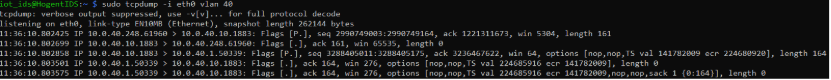
\includegraphics[width=1\textwidth]{../graphics/Proxmox/vlan40Verkeer.png}
    \caption{Verkeer op VLAN 40.}
    \label{fig:vlan40-verkeer}
\end{figure}

\subsubsection{Suricata installatie en configuratie}

Suricata wordt op de Raspberry Pi geïnstalleerd als een Intrusion Detection System (IDS) om het netwerkverkeer in real-time te inspecteren op bekende aanvalspatronen. Voor de detectie-capaciteit is gekozen voor de implementatie van de standaard enterprise-regelset (Emerging Threats), maar we stellen ook aangepaste regelsets samen die specifiek zijn ontworpen om IoT-aanvallen te testen.
Om ons IDS volledig af te stemmen op de analyse van ons netwerkverkeer, hebben we het configuratiebestand van Suricata aangepast. Zoals te zien is in Listing \ref{lst:suricata-conf}, is \texttt{HOME\_NET} gedefinieerd met beide subnetten, en zijn de specifieke rollen van de Proxmox-servers en de IoT-clients als variabelen ingesteld.

\begin{listing}[H]
\begin{minted}[breaklines, linenos, frame=lines]{yaml}
vars:
  
  address-groups:
    HOME_NET: "[192.168.1.0/24,10.0.40.0/24]"
    EXTERNAL_NET: "!$HOME_NET"

    # Proxmox Services
    MQTT_SERVERS: "[10.0.40.10]"
    ZIGBEE_BRIDGE: "[10.0.40.15]"
    HOMEASSISTANT: "[192.168.1.57]"

    # WIFI DHCP POOL
    IOT_CLIENTS: "[10.0.40.100-10.0.40.250]"
\end{minted}
\caption{Aangepaste address-groups variabelen in \texttt{suricata.yaml} voor netwerkspecifieke detectie.}
\label{lst:suricata-conf}
\end{listing}

Door deze variabelen te definiëren, kunnen we Suricata zeggen om onderscheid te maken tussen intern en extern verkeer. Later zullen we deze variabelen gebruiken om onze aangepaste IoT-regels te schrijven.

\subsubsection{Zeek installatie en configuratie}


We hebben Zeek ingesteld als een standalone node die het verkeer op \texttt{eth0} analyseert. Aangezien Zeek anders werkt dan de traditionele netwerkbeveiligingssystemen, moet het systeem eerst het netwerkverkeer leren om een baseline te creëren van hoe normaal verkeer eruitziet. Net als bij Suricata hebben we de relevante IP-adressen en subnetten gedefinieerd die verwijzen naar ons IoT-netwerk en de bijbehorende diensten. Deze configuratie verrijkt de uiteindelijke logbestanden die door Zeek worden gegenereerd, wat het identificeren van specifieke actoren tijdens de data-analyse aanzienlijk vereenvoudigt. De opgeschoonde configuraties worden weergegeven in Listing \ref{lst:zeek-node} en Listing \ref{lst:zeek-networks}.


\begin{listing}[H]
\begin{minted}[breaklines, linenos, frame=lines]{ini}
[zeek]
type=standalone
host=localhost
interface=eth0
\end{minted}
\caption{Interface- en modusconfiguratie van Zeek in \texttt{node.cfg}.}
\label{lst:zeek-node}
\end{listing}

\begin{listing}[H]
\begin{minted}[breaklines, linenos, frame=lines]{text}
# IoT Subnet
10.0.40.0/24        IoT_environment
10.0.40.10/32       MosquitoMQTT
10.0.40.15/32       Zigbee2MQTT

# LAN and Proxmox Services
192.168.1.0/24      LAN_Management
192.168.1.55/32     MikrotikRouter
192.168.1.57/32     HomeAssistant
192.168.1.58/32     IDS
192.168.1.200/32    ProxmoxServer
\end{minted}
\caption{Definitie van netwerksegmenten en hosts in \texttt{networks.cfg}.}
\label{lst:zeek-networks}
\end{listing}



Zoals eerder vastgesteld, genereert Zeek specifieke logbestanden om een gedetailleerde netwerkanalyse mogelijk te maken. Aangezien de IoT-apparaten in deze setup communiceren via het MQTT-protocol, creëert Zeek automatisch een \texttt{mqtt\_publish.log} bestand. Dit bestand registreert de specifieke payloads die naar de lokale broker worden gepubliceerd, waarvan een voorbeeld wordt getoond in Listing~\ref{lst:zeek-mqtt-logs}.


\begin{listing}[H]
\begin{minted}[breaklines, linenos, frame=lines, fontsize=\scriptsize]{text}
iot_ids@HogentIDS:~ $ sudo cat /opt/zeek/logs/current/mqtt_publish.log | /opt/zeek/bin/zeek-cut id.orig_h id.resp_h topic payload
10.0.40.15      10.0.40.10      zigbee2mqtt/bridge/logging      {"level":"info","message":"z2m:mqtt: MQTT publish: topic 'zigbee2mqtt/0x58e6c5fffe1c6f24', payload '
10.0.40.15      10.0.40.10      zigbee2mqtt/bridge/logging      {"level":"info","message":"z2m:mqtt: MQTT publish: topic 'zigbee2mqtt/0x58e6c5fffe1c6f24', payload '
10.0.40.1       10.0.40.10      zigbee2mqtt/0x58e6c5fffe1c6f24  \x02\x0b\x01{"linkquality":229,"temperature":20}
10.0.40.15      10.0.40.10      zigbee2mqtt/0x58e6c5fffe1c6f24  {"linkquality":229,"temperature":20}
192.168.1.57    10.0.40.10      zigbee2mqtt/0x58e6c5fffe1c6f24  \x02\x0b\x01{"linkquality":229,"temperature":20}
10.0.40.248     10.0.40.10      iot/esp32s3/telemetry   {"seq":139245,"device_id":"ESP32-S3-N16R8","uptime_sec":696242,"free_heap":258896,"free_psram":83814
10.0.40.1       10.0.40.10      iot/esp32s3/telemetry   \x02\x0b\x01{"seq":139245,"device_id":"ESP32-S3-N16R8","uptime_sec":696242,"free_heap":258896,"free_psram":83
192.168.1.57    10.0.40.10      iot/esp32s3/telemetry   \x02\x0b\x01{"seq":139245,"device_id":"ESP32-S3-N16R8","uptime_sec":696242,"free_heap":258896,"free_psram":83
\end{minted}
\caption{Zeek-cut output van MQTT logs.}
\label{lst:zeek-mqtt-logs}
\end{listing}



\subsection{MikroTik hAP ac lite configuratie}

De MikroTik hAP ac lite werkt binnen deze infrastructuur als de draadloze toegangspunt (WAP) voor de IoT-omgeving. De initiële configuratie en het beheer van de router worden uitgevoerd via de grafische Winbox-beheeromgeving (Figuur~\ref{fig:winboxpage}). De belangrijkste taak van deze router is het scheiden van het IoT-verkeer van het reguliere beheernetwerk door middel van VLAN 40. 
\begin{figure}[H]
    \centering
    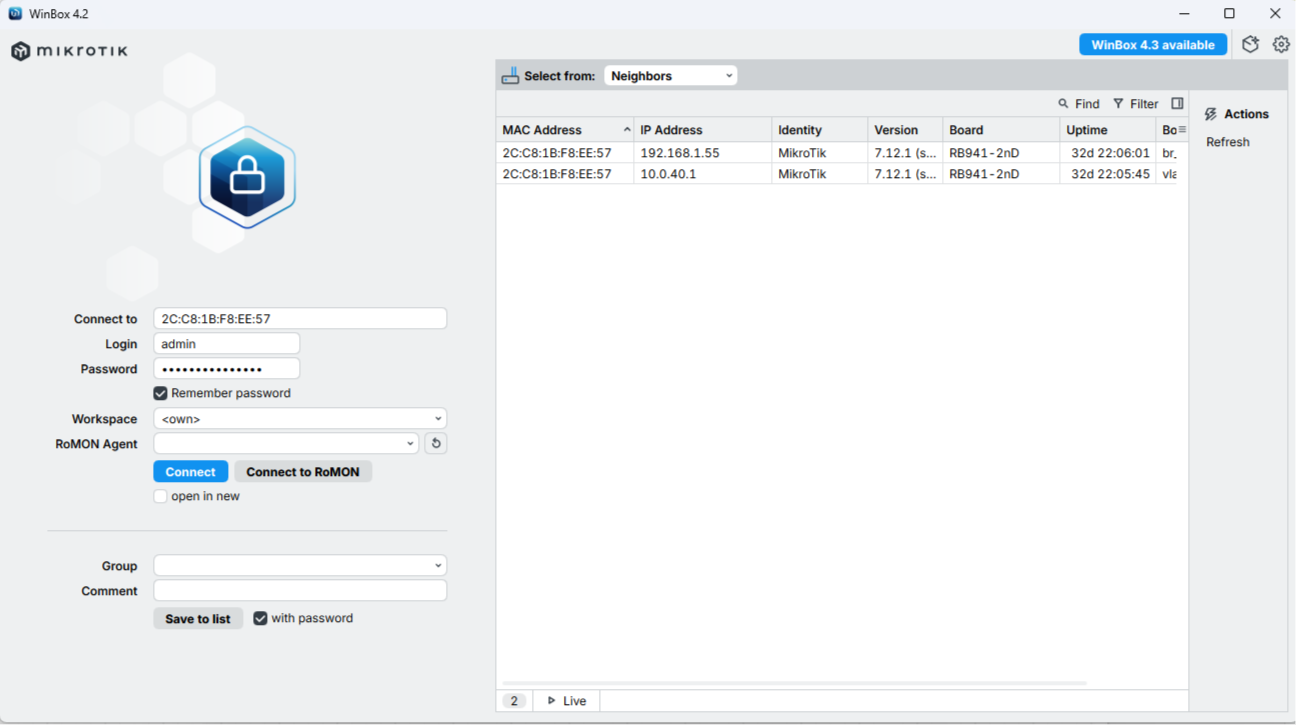
\includegraphics[width=1\textwidth]{../graphics/Proxmox/winboxplatform.png}
    \caption{WinBox 4.2 inlogpagina.}
    \label{fig:winboxpage}
\end{figure}


Via Winbox is een bridge (\texttt{br\_lan}) aangemaakt met VLAN-filtering ingeschakeld. Het fysieke LAN-poort (\texttt{ether1}) en de WiFi-interface (\texttt{wlan1}) zijn aan deze bridge gekoppeld, waarbij de WiFi-interface direct is toegewezen aan VLAN 40 (PVID 40). De IoT-apparaten verbinden via een beveiligd WPA2-PSK netwerk met de SSID \texttt{Bachelorproef\_IoT}. 
De volledige geëxporteerde configuratie zonder gevoelige credentials is weergegeven in Listing \ref{lst:mikrotik-config}.


\begin{listing}[H]
\begin{minted}[breaklines, linenos, frame=lines]{text}
# 1970-01-29 11:14:42 by RouterOS 7.12.1
# software id = 2KKX-GRFF
# model = RB941-2nD
# serial number = D0550E6F8658
/interface bridge
add name=br_lan vlan-filtering=yes
/interface vlan
add interface=br_lan name=vlan40 vlan-id=40
/interface wireless security-profiles
set [ find default=yes ] supplicant-identity=MikroTik
add authentication-types=wpa2-psk mode=dynamic-keys name=iot_crypto supplicant-identity=""
/interface wireless
set [ find default-name=wlan1 ] disabled=no mode=ap-bridge security-profile=iot_crypto ssid=Bachelorproef_IoT
/ip pool
add name=dhcp_pool0 ranges=10.0.40.100-10.0.40.250
/ip dhcp-server
add address-pool=dhcp_pool0 interface=vlan40 lease-time=1d name=dhcp1
/interface bridge port
add bridge=br_lan interface=ether1
add bridge=br_lan interface=wlan1 pvid=40
/interface bridge vlan
add bridge=br_lan tagged=br_lan,ether1 vlan-ids=40
/ip address
add address=10.0.40.1/24 interface=vlan40 network=10.0.40.0
add address=192.168.1.55/24 interface=br_lan network=192.168.1.0
/ip dhcp-server network
add address=10.0.40.0/24 dns-server=1.1.1.1 gateway=10.0.40.1
/ip firewall filter
add action=accept chain=forward dst-address=10.0.40.0/24 log=yes src-address=192.168.1.0/24
/ip firewall nat
add action=masquerade chain=srcnat src-address=10.0.40.0/24
add action=masquerade chain=srcnat dst-address=10.0.40.0/24
/ip route
add disabled=no dst-address=0.0.0.0/0 gateway=192.168.1.1 routing-table=main suppress-hw-offload=no
/system note
set show-at-login=no
\end{minted}
\caption{Geëxporteerde RouterOS configuratie van de MikroTik hAP ac lite voor VLAN 40 scheiding.}
\label{lst:mikrotik-config}
\end{listing}





\chapter{\IfLanguageName{dutch}{Ontwikkeling van custom rules}{Ontwikkeling van custom rules}}%
\label{ch:Ontwikkeling van custom rules}

\section{Suricata custom rules}

Voordat we beginnen met het schrijven van regels voor onze IoT-omgeving, moeten we de syntaxis van Suricata-regels begrijpen.
Een Suricata-regel bestaat uit twee belangrijke logische componenten: de \textit{regelkop} (die de actie, het protocol, de IP-adressen, de poorten en de netwerkrichting definieert) en de \textit{regelopties} (die tussen haakjes staan en de specifieke overeenkomingscriteria en metagegevens bevatten) \autocite{SuricataRulesDiff2024}. De algemene structuur is als volgt gedefinieerd:

\begin{verbatim}
[actie] [protocol] [bron_IP] [bron_poort] -> [doel_IP] [doel_poort] ([opties])
\end{verbatim}

Binnen deze bachelorproef is gebruikgemaakt van de actie \texttt{alert}, waarmee Suricata bij een match een waarschuwing genereert en wegschrijft naar \texttt{fast.log} en het gestructureerde \texttt{eve.json}.

\subsection{Protocol Afwijkingen en Fuzzing}
De eerste twee regels richten zich op abnormaal gedrag binnen de verwachte MQTT-communicatie. Omdat MQTT een specifiek eigen protocol heeft op poort 1883, mag hier normaal gesproken geen standaard HTTP-verkeer of onleesbare data verschijnen.

\begin{listing}[H]
\begin{minted}[breaklines, linenos, frame=lines, fontsize=\small]{text}
# Protocol Mismatch on MQTT Port
alert tcp any any -> $MQTT_SERVERS 1883 (msg:"IoT-IDS: HTTP Protocol Mismatch Detected on MQTT Port 1883"; flow:to_server; content:"GET "; depth:4; sid:1000002; rev:3;)
\end{minted}
\caption{Suricata-regel voor het detecteren van een protocol-mismatch op de MQTT-poort.}
\label{lst:suricata-rule-http}
\end{listing}

Listing \ref{lst:suricata-rule-http} is ontworpen om een veelvoorkomende scanning- of misconfiguratiefout op te sporen. Het inspecteert de eerste vier bytes (\texttt{depth:4}) van het TCP-pakket richting de broker. Als dit overeenkomt met een HTTP \texttt{GET } verzoek, genereert het IDS een alert. MQTT gebruikt geen HTTP-commando's; het verschijnen hiervan duidt op een verkeerd geconfigureerde client, een portscan, of een kwaadaardige poging om de broker te misleiden.

\begin{listing}[H]
\begin{minted}[breaklines, linenos, frame=lines, fontsize=\small]{text}
# Buffer Overflow / Repeated Pattern in MQTT
alert tcp any any -> $MQTT_SERVERS 1883 (msg:"IoT-IDS: Malformed MQTT Payload / Oversized Buffer Detected"; flow:to_server; content:"AAAAAAAAAAAAAAAA"; sid:1000003; rev:4;)
\end{minted}
\caption{Suricata-regel voor het detecteren van een mogelijke buffer overflow.}
\label{lst:suricata-rule-buffer}
\end{listing}

De regel in Listing \ref{lst:suricata-rule-buffer} fungeert als een eenvoudige anomaliedetectie voor malafide payloads. Het zoekt naar een herhaald patroon van de letter "A". Hoewel dit een specifiek patroon is, is het in praktijktests een effectieve manier om foutief geprogrammeerde IoT-apparaten (die garbage data verzenden) of actieve fuzzing-aanvallen te identificeren waarbij een aanvaller probeert de buffer van de MQTT-broker te overschrijden (buffer overflow).

\subsection{Denial of Service (DoS) Bescherming}
Naast het inspecteren van de payload, is het monitoren van het verkeersvolume naar de MQTT-broker cruciaal om de beschikbaarheid van het IoT-netwerk te garanderen.

\begin{listing}[H]
\begin{minted}[breaklines, linenos, frame=lines, fontsize=\small]{text}
# High-Frequency Burst targeting MQTT Broker
alert tcp any any -> $MQTT_SERVERS 1883 (msg:"IoT-IDS: High-Frequency Connection Burst to MQTT Broker"; flags:S,12; threshold: type threshold, track by_src, count 10, seconds 2; sid:1000010; rev:1;)
\end{minted}
\caption{Suricata-regel voor het detecteren van een high-frequency SYN-flood (DoS).}
\label{lst:suricata-rule-dos}
\end{listing}

De regel in Listing \ref{lst:suricata-rule-dos} is geïmplementeerd om Denial of Service (DoS) aanvallen te detecteren. In plaats van elk afzonderlijk pakket te loggen (wat de logbestanden zou overspoelen), maakt deze regel gebruik van Suricata's ingebouwde \texttt{threshold} functie. Het systeem houdt TCP-SYN pakketten (\texttt{flags:S,12}) bij per bron-IP (\texttt{track by\_src}). Pas wanneer een enkel IP-adres binnen een tijdspanne van twee seconden (\texttt{seconds 2}) meer dan 10 nieuwe connectieverzoeken (\texttt{count 10}) verzendt, wordt er een enkele waarschuwing gegenereerd. Dit voorkomt log-saturatie en wijst direct op een mogelijke SYN-flood aanval gericht op de broker.


\section{Zeek custom scripts}

In tegenstelling tot Suricata, dat werkt op basis van statische signatuurregels, maakt Zeek gebruik van een \textit{event-driven} scripttaal om netwerkverkeer te analyseren. Hoewel Zeek standaard al waarschuwingen kan genereren bij afwijkend netwerkgedrag, kunnen wij met behulp van custom Zeek-scripts ook proactief eigen detectielogica toepassen.

Voordat we deze aangepaste scripts schrijven, is het belangrijk om te weten dat Zeek-scripts uit twee onderdelen bestaan: de \textit{module- en export-definities} (waarbij custom notificatietypen en configureerbare drempelwaarden worden gedeclareerd) en de \textit{event-handlers} (functies die automatisch worden geactiveerd wanneer Zeek een specifieke netwerkgebeurtenis waarneemt). De algemene opzet van de module-definities voor deze bachelorproef is als volgt:

\begin{listing}[H]
\begin{minted}[breaklines, linenos, frame=lines, fontsize=\small]{zeek}
@load base/protocols/http

module CustomIoT;

export {
    # Definieer custom notice types
    redef enum Notice::Type += {
        HTTP_On_MQTT_Port,
        Malformed_MQTT_Payload,
        MQTT_Syn_Flood
    };

    # Configureerbare drempelwaarden
    const syn_threshold = 10 &redef;
    const syn_interval = 2sec &redef;
}
\end{minted}
\caption{Basisconfiguratie en variabele declaraties van de \texttt{CustomIoT} module in Zeek.}
\label{lst:zeek-module}
\end{listing}


Binnen deze bachelorproef is gebruikgemaakt van de \texttt{NOTICE} functie, het Zeek-equivalent van een Suricata \texttt{alert}. Wanneer een event overeenkomt met onze criteria, genereert Zeek een waarschuwing en schrijft deze weg naar het gestructureerde \texttt{notice.log} bestand.

\subsection{Implementatie van de equivalente detectieregels in Zeek}

In de vorige secties werd er toegelicht welke signatureregels voor Suricata zijn opgesteld. Om onnodige herhaling in dit document te voorkomen, wordt de theoretische logica achter deze detecties hier niet opnieuw behandeld. In plaats daarvan ligt de focus op de architecturale vertaling van deze statische regels naar event-driven scripts voor Zeek.
Hoewel de scripttaal van Zeek complexer is en meer op een programmeertaal lijkt, kunnen netwerkbeheerders meer controle hebben van hun netwerk. Door te luisteren naar specifieke netwerk events en gebruik te maken van uitgebreide gegevenstype, is zeek in staat om dezelfde aanvalsscenario’s op te sporen en alarmeren. De volledige, gecombineerde \texttt{CustomIoT}-module die deze drie scenario’s afhandelt, wordt weergegeven in Listing~\ref{lst:zeek-full-script}.


\begin{listing}[H]
\begin{minted}[breaklines, linenos, frame=lines, fontsize=\small]{zeek}
# Aanvalsscenario 1: Protocol Mismatch (HTTP op MQTT)
event http_request(c: connection, method: string, original_URI: string,
                   http_version: string, user_agent: string) &priority=-5 {
    if ( c$id$resp_p == 1883/tcp ) {
        NOTICE([$note=CustomIoT::HTTP_On_MQTT_Port,
                $msg=fmt("Protocol Mismatch: HTTP %s request naar MQTT poort 1883", method),
                $conn=c,
                $identifier=cat(c$id$orig_h)]);
    }
}

# Aanvalsscenario 2: Malformed Payload (AAAA patroon)
event tcp_packet(c: connection, is_orig: bool, flags: string,
                 seq: count, ack: count, len: count, payload: string) {
    if ( c$id$resp_p == 1883/tcp && is_orig ) {
        if ( /AAAAAAAAAAAAAAAA/ in payload ) {
            NOTICE([$note=CustomIoT::Malformed_MQTT_Payload,
                    $msg="Malformed payload / Buffer overflow patroon gedetecteerd",
                    $conn=c,
                    $identifier=cat(c$id$orig_h)]);
        }
    }
}

# Aanvalsscenario 3: SYN Flood / High-Frequency Burst
global Track_Syn: table[addr] of count &write_expire=CustomIoT::syn_interval;

event new_connection(c: connection) {
    if ( c$id$resp_p == 1883/tcp ) {
        if ( c$id$orig_h !in Track_Syn ) {
            Track_Syn[c$id$orig_h] = 0;
        }
        Track_Syn[c$id$orig_h] += 1;
        if ( Track_Syn[c$id$orig_h] == CustomIoT::syn_threshold ) {
            NOTICE([$note=CustomIoT::MQTT_Syn_Flood,
                    $msg=fmt("High-Frequency Burst: %d verbindingen in %s naar MQTT poort van %s",
                             CustomIoT::syn_threshold, CustomIoT::syn_interval, c$id$orig_h),
                    $conn=c,
                    $identifier=cat(c$id$orig_h)]);
        }
    }
}
\end{minted}
\caption{Het volledige \texttt{CustomIoT.zeek} script ter implementatie van de drie voorafgedefinieerde aanvalsscenario's.}
\label{lst:zeek-full-script}
\end{listing}

\chapter{\IfLanguageName{dutch}{Aanvalsscenario's en actieve validatie}{Aanvalsscenario's en actieve validatie}}%
\label{ch:Aanvalsscenario's en actieve validatie}
Om de effectiviteit van de geconfigureerde detectiesystemen te valideren, worden er gecontroleerde penetratietesten uitgevoerd op het IoT-netwerk. Er worden drie specifieke aanvalsscenario's getest die direct aansluiten bij de geschreven custom rules en scripts: een Denial of Service (SYN Flood), een malformed payload (buffer overflow patroon) en een protocol mismatch (HTTP op de MQTT-poort).

Voor het genereren van dit aanvalsverkeer is een eigen Python-script ontwikkeld dat gebruikmaakt van de \texttt{Scapy}  en het \texttt{Socket} bibliotheek. Met Scapy is het mogelijk om netwerkpakketten op bit-niveau te creëren, wat zorgt voor een zeer precieze simulatie van de aanvallen. De scenario’s worden uitgevoerd vanaf een fysiek computer die aangesloten is op het IoT-netwerk. Omdat het netwerkverkeer via een SPAN-poort op de switch wordt gespiegeld naar de Raspberry Pi, krijgt onze NIDS het kwaadaardig verkeer ook te zien.

\subsection{Validatie van Suricata custom rules}
Om te verifiëren dat de aangepaste Suricata-regels correct functioneren, kan het commando \texttt{tail -f /var/log/suricata/fast.log} worden uitgevoerd. Dit biedt een live weergave van de alerts die door Suricata worden gedetecteerd tijdens de penetratietesten.



\begin{listing}[H]
\begin{minted}[breaklines, linenos, frame=lines, fontsize=\footnotesize]{text}
iot_ids@HogentIDS:~ $ sudo tail -f /var/log/suricata/fast.log 
04/21/2026-11:46:35.004549  [**] [1:1000002:3] IoT-IDS: HTTP Protocol Mismatch Detected on MQTT Port 1883 [**] [Classification: (null)] [Priority: 3] {TCP} 10.0.40.249:64247 -> 10.0.40.10:1883
04/21/2026-11:46:35.004764  [**] [1:1000002:3] IoT-IDS: HTTP Protocol Mismatch Detected on MQTT Port 1883 [**] [Classification: (null)] [Priority: 3] {TCP} 10.0.40.249:64247 -> 10.0.40.10:1883
04/21/2026-11:46:37.777019  [**] [1:1000003:4] IoT-IDS: Malformed MQTT Payload / Oversized Buffer Detected [**] [Classification: (null)] [Priority: 3] {TCP} 10.0.40.249:64248 -> 10.0.40.10:1883
04/21/2026-11:46:37.777019  [**] [1:2229010:1] SURICATA MQTT malformed traffic [**] [Classification: Generic Protocol Command Decode] [Priority: 3] {TCP} 10.0.40.249:64248 -> 10.0.40.10:1883
04/21/2026-11:46:37.777081  [**] [1:1000003:4] IoT-IDS: Malformed MQTT Payload / Oversized Buffer Detected [**] [Classification: (null)] [Priority: 3] {TCP} 10.0.40.249:64248 -> 10.0.40.10:1883
04/21/2026-11:46:37.777081  [**] [1:2229010:1] SURICATA MQTT malformed traffic [**] [Classification: Generic Protocol Command Decode] [Priority: 3] {TCP} 10.0.40.249:64248 -> 10.0.40.10:1883
04/21/2026-11:46:42.279527  [**] [1:1000010:1] IoT-IDS: High-Frequency Connection Burst to MQTT Broker [**] [Classification: (null)] [Priority: 3] {TCP} 10.0.40.249:64256 -> 10.0.40.10:1883
04/21/2026-11:46:42.279834  [**] [1:1000010:1] IoT-IDS: High-Frequency Connection Burst to MQTT Broker [**] [Classification: (null)] [Priority: 3] {TCP} 10.0.40.249:64257 -> 10.0.40.10:1883
\end{minted}
\caption{Uitvoer van \texttt{fast.log} tijdens de actieve validatie van de drie custom Suricata-regels.}
\label{lst:suricata-fast-log}

\end{listing}

Zoals te zien in Listing \ref{lst:suricata-fast-log}, werden alle drie regels succesvol getriggerd tijdens de aanval. Het is ook interessant om op te merken dat niet alleen onze aangepaste regels werden geactiveerd, maar dat tegelijkertijd ook de standaard MQTT-protocoldecoder van Suricata (SID 2229010) een waarschuwing heeft gegenereerd.



\subsection{Validatie van Zeek custom scripts}
Om de werking van de aangepaste Zeek-scripts te valideren, kan de gegenereerde \texttt{notice.log} worden geanalyseerd. Met behulp van het \texttt{zeek-cut} commando kan deze logfile worden geparseerd en gefilterd, zodat alleen de meest relevante metagegevens (zoals bron-IP, bestemmings-IP, het type notificatie en de tijdstempel) overzichtelijk worden weergegeven.

\begin{listing}[H]
\begin{minted}[breaklines, linenos, frame=lines, fontsize=\footnotesize]{text}
iot_ids@HogentIDS:~ $ sudo cat /opt/zeek/logs/current/notice.log | /opt/zeek/bin/zeek-cut id.orig_h id.resp_h note msg ts
10.0.40.249     10.0.40.10      CustomIoT::HTTP_On_MQTT_Port    Protocol Mismatch: HTTP GET request naar MQTT poort 1883        1787323935.694449
10.0.40.249     10.0.40.10      CustomIoT::Malformed_MQTT_Payload       Malformed payload / Buffer overflow patroon gedetecteerd        1787323940.807833
10.0.40.249     10.0.40.10      CustomIoT::MQTT_Syn_Flood       High-Frequency Burst: 10 verbindingen in 2.0 secs naar MQTT poort van 10.0.40.249       1787323944.638297
\end{minted}
\caption{Uitvoer van \texttt{notice.log} tijdens de actieve validatie van Zeek custom scripts.}
\label{lst:zeek-notice-log}
\end{listing}




\chapter{\IfLanguageName{dutch}{Verzamelen en analyseren van meetgegevens}{Verzamelen en analyseren van meetgegevens}}%
\label{ch:Verzamelen en analyseren van meetgegevens}
In dit hoofdstuk verzamelen wij kwantitatieve data over de prestaties van Suricata en Zeek op de Raspberry Pi 4. Om de impact van beide Intrusion Detection Systems (IDS) op de systeembronnen objectief te beoordelen, is een gestructureerde meetmethodologie opgezet. De verzamelde data worden verkregen tijdens opeenvolgende sessies van 30 minuten. We visualiseren drie netwerktoestanden gedurende onze verzameling (idle, baseline en attack) om een representatief antwoord te bieden op de centrale onderzoeksvraag.



\section{Meetmethodologie}
Het belangrijkste doel is om gegevens te verzamelen over het resourcegebruik van beide IDS’en wanneer ze als zelfstandig apparaat draaien. Hiervoor is een Python-script geschreven, dat zelfstandig op de achtergrond op de Raspberry Pi draait en na afloop een CSV-bestand aanmaakt.


\subsection{python-script voor het verzamelen van metrieken}
Het script maakt gebruik van \texttt{psutil} om direct op kernel-niveau procesinformatie te verkrijgen van de specifieke PID’s (Process Identifiers) van Suricata en Zeek. Het script monitort het CPU-verbruik, het gebruik van fysieke RAM en het totale systeemgeheugen. Deze gegevens worden in realtime opgeslagen in een gestructureerd CSV-bestand om deze later te kunnen analyseren.

De broncode van het script is hieronder weergegeven:


\begin{minted}[breaklines, linenos, frame=lines, fontsize=\footnotesize]{python}
import csv
import os
import sys
import time
import psutil

# Supported target IDS engines
TARGET_ENGINES = ["suricata", "zeek"]
SAMPLE_INTERVAL = 1.0


def get_target_processes(engine_names):
    """Finds and returns persistent psutil.Process objects matching any target engine name."""
    procs = []
    for proc in psutil.process_iter(["pid", "name"]):
        try:
            proc_name = proc.info["name"]
            if proc_name and any(
                engine.lower() in proc_name.lower() for engine in engine_names
            ):
                procs.append(proc)
        except (psutil.NoSuchProcess, psutil.AccessDenied):
            continue
    return procs


def main():
    # 1. Parse Output File Parameter
    if len(sys.argv) > 1:
        output_file = sys.argv[1]
    else:
        output_file = "ids_metrics.csv"
        print(f"[*] No output file specified. Defaulting to '{output_file}'.")

    # Ensure output directory exists if a path like /output/file.csv was passed
    output_dir = os.path.dirname(output_file)
    if output_dir and not os.path.exists(output_dir):
        os.makedirs(output_dir, exist_ok=True)

    # 2. Find Active IDS Processes (Suricata or Zeek)
    procs = get_target_processes(TARGET_ENGINES)
    if not procs:
        print(
            f"[!] Error: No active processes found for engines: {', '.join(TARGET_ENGINES)}"
        )
        sys.exit(1)

    # Group detected process names for clear output logging
    detected_names = set(p.name() for p in procs)
    pids = [p.pid for p in procs]

    # 3. Initialize CPU measurement baseline for each process
    for p in procs:
        try:
            p.cpu_percent(interval=None)
        except (psutil.NoSuchProcess, psutil.AccessDenied):
            pass

    print(
        f"[*] Monitoring Active IDS: {', '.join(detected_names)} (PIDs: {pids})"
    )
    print(f"[*] Writing telemetry to: {output_file}")
    time.sleep(1)  # Baseline time interval window

    # 4. Monitoring Loop
    with open(output_file, mode="w", newline="") as file:
        writer = csv.writer(file)
        writer.writerow(
            ["Timestamp_Sec", "CPU_Percent", "RAM_MB", "RAM_Percent"]
        )

        start_time = time.time()
        try:
            while True:
                # Filter out any terminated processes
                procs = [p for p in procs if p.is_running()]
                if not procs:
                    print("\n[!] All monitored IDS processes have terminated.")
                    break

                total_cpu = 0.0
                total_ram_mb = 0.0
                total_ram_percent = 0.0

                for proc in procs:
                    try:
                        total_cpu += proc.cpu_percent(interval=None)
                        mem_info = proc.memory_info()
                        total_ram_mb += mem_info.rss / (1024 * 1024)
                        total_ram_percent += proc.memory_percent()
                    except (psutil.NoSuchProcess, psutil.AccessDenied):
                        continue

                elapsed_time = round(time.time() - start_time, 2)

                writer.writerow(
                    [
                        elapsed_time,
                        round(total_cpu, 2),
                        round(total_ram_mb, 2),
                        round(total_ram_percent, 2),
                    ]
                )
                file.flush()

                time.sleep(SAMPLE_INTERVAL)

        except KeyboardInterrupt:
            print(f"\n[*] Monitoring stopped. Data saved to '{output_file}'.")

if __name__ == "__main__":
    main()
\end{minted}


\section{Meetomstandigheden}
De prestatiemetingen zijn uitgevoerd tijdens opeenvolgende testsessies van 30 minuten per scenario. Dit tijdsbestek is gekozen om kortstondige fluctuaties (spikes) uit te middelen en de stabiliteit van de systemen op lange termijn aan te tonen. 
De metingen vonden plaats onder drie specifieke en gecontroleerde omstandigheden:
\begin{enumerate}
    \item \textbf{Rusttoestand (Idle-status):} De Raspberry Pi is actief en de NIDS draait, maar er wordt geen netwerkverkeer beluisterd op de interface. Dit scenario dient om het basisverbruik van de engines te bepalen.
    \item \textbf{Normale Operationele Toestand (Baseline-status):} De NIDS beluisterd de SPAN-link naar het netwerkverkeer binnen VLAN 40. Dit verkeer bevat het continue stroom van MQTT-berichten en Tuya-toestellen.
    \item \textbf{Aanvalstoestand (Stress-status):} De NIDS beluisterd en gebruiken de custom rules en scripts om actieve cyberaanvallen, die elke 60 seconden worden gelanceerd, te detecteren.
\end{enumerate}

\section{Meetresultaten}
In dit hoofdstuk worden de gegevens weergegeven die tijdens elke sessie zijn verzameld. Om een logische opbouw te garanderen, volgt de presentatie van de resultaten de eerder gedefinieerde meetomstandigheden.



\subsubsection{Rusttoestand (idle)}
Tijdens de initiële rusttoestand (idle-status) is het systeemverbruik van beide IDS gemeten terwijl er geen netwerkverkeer werd gegenereerd. De resultaten zijn gevisualiseerd in Figuur~\ref{fig:suricata_idle} voor Suricata en Figuur~\ref{fig:zeek_idle} voor Zeek.



\begin{figure}[H]
    \centering
    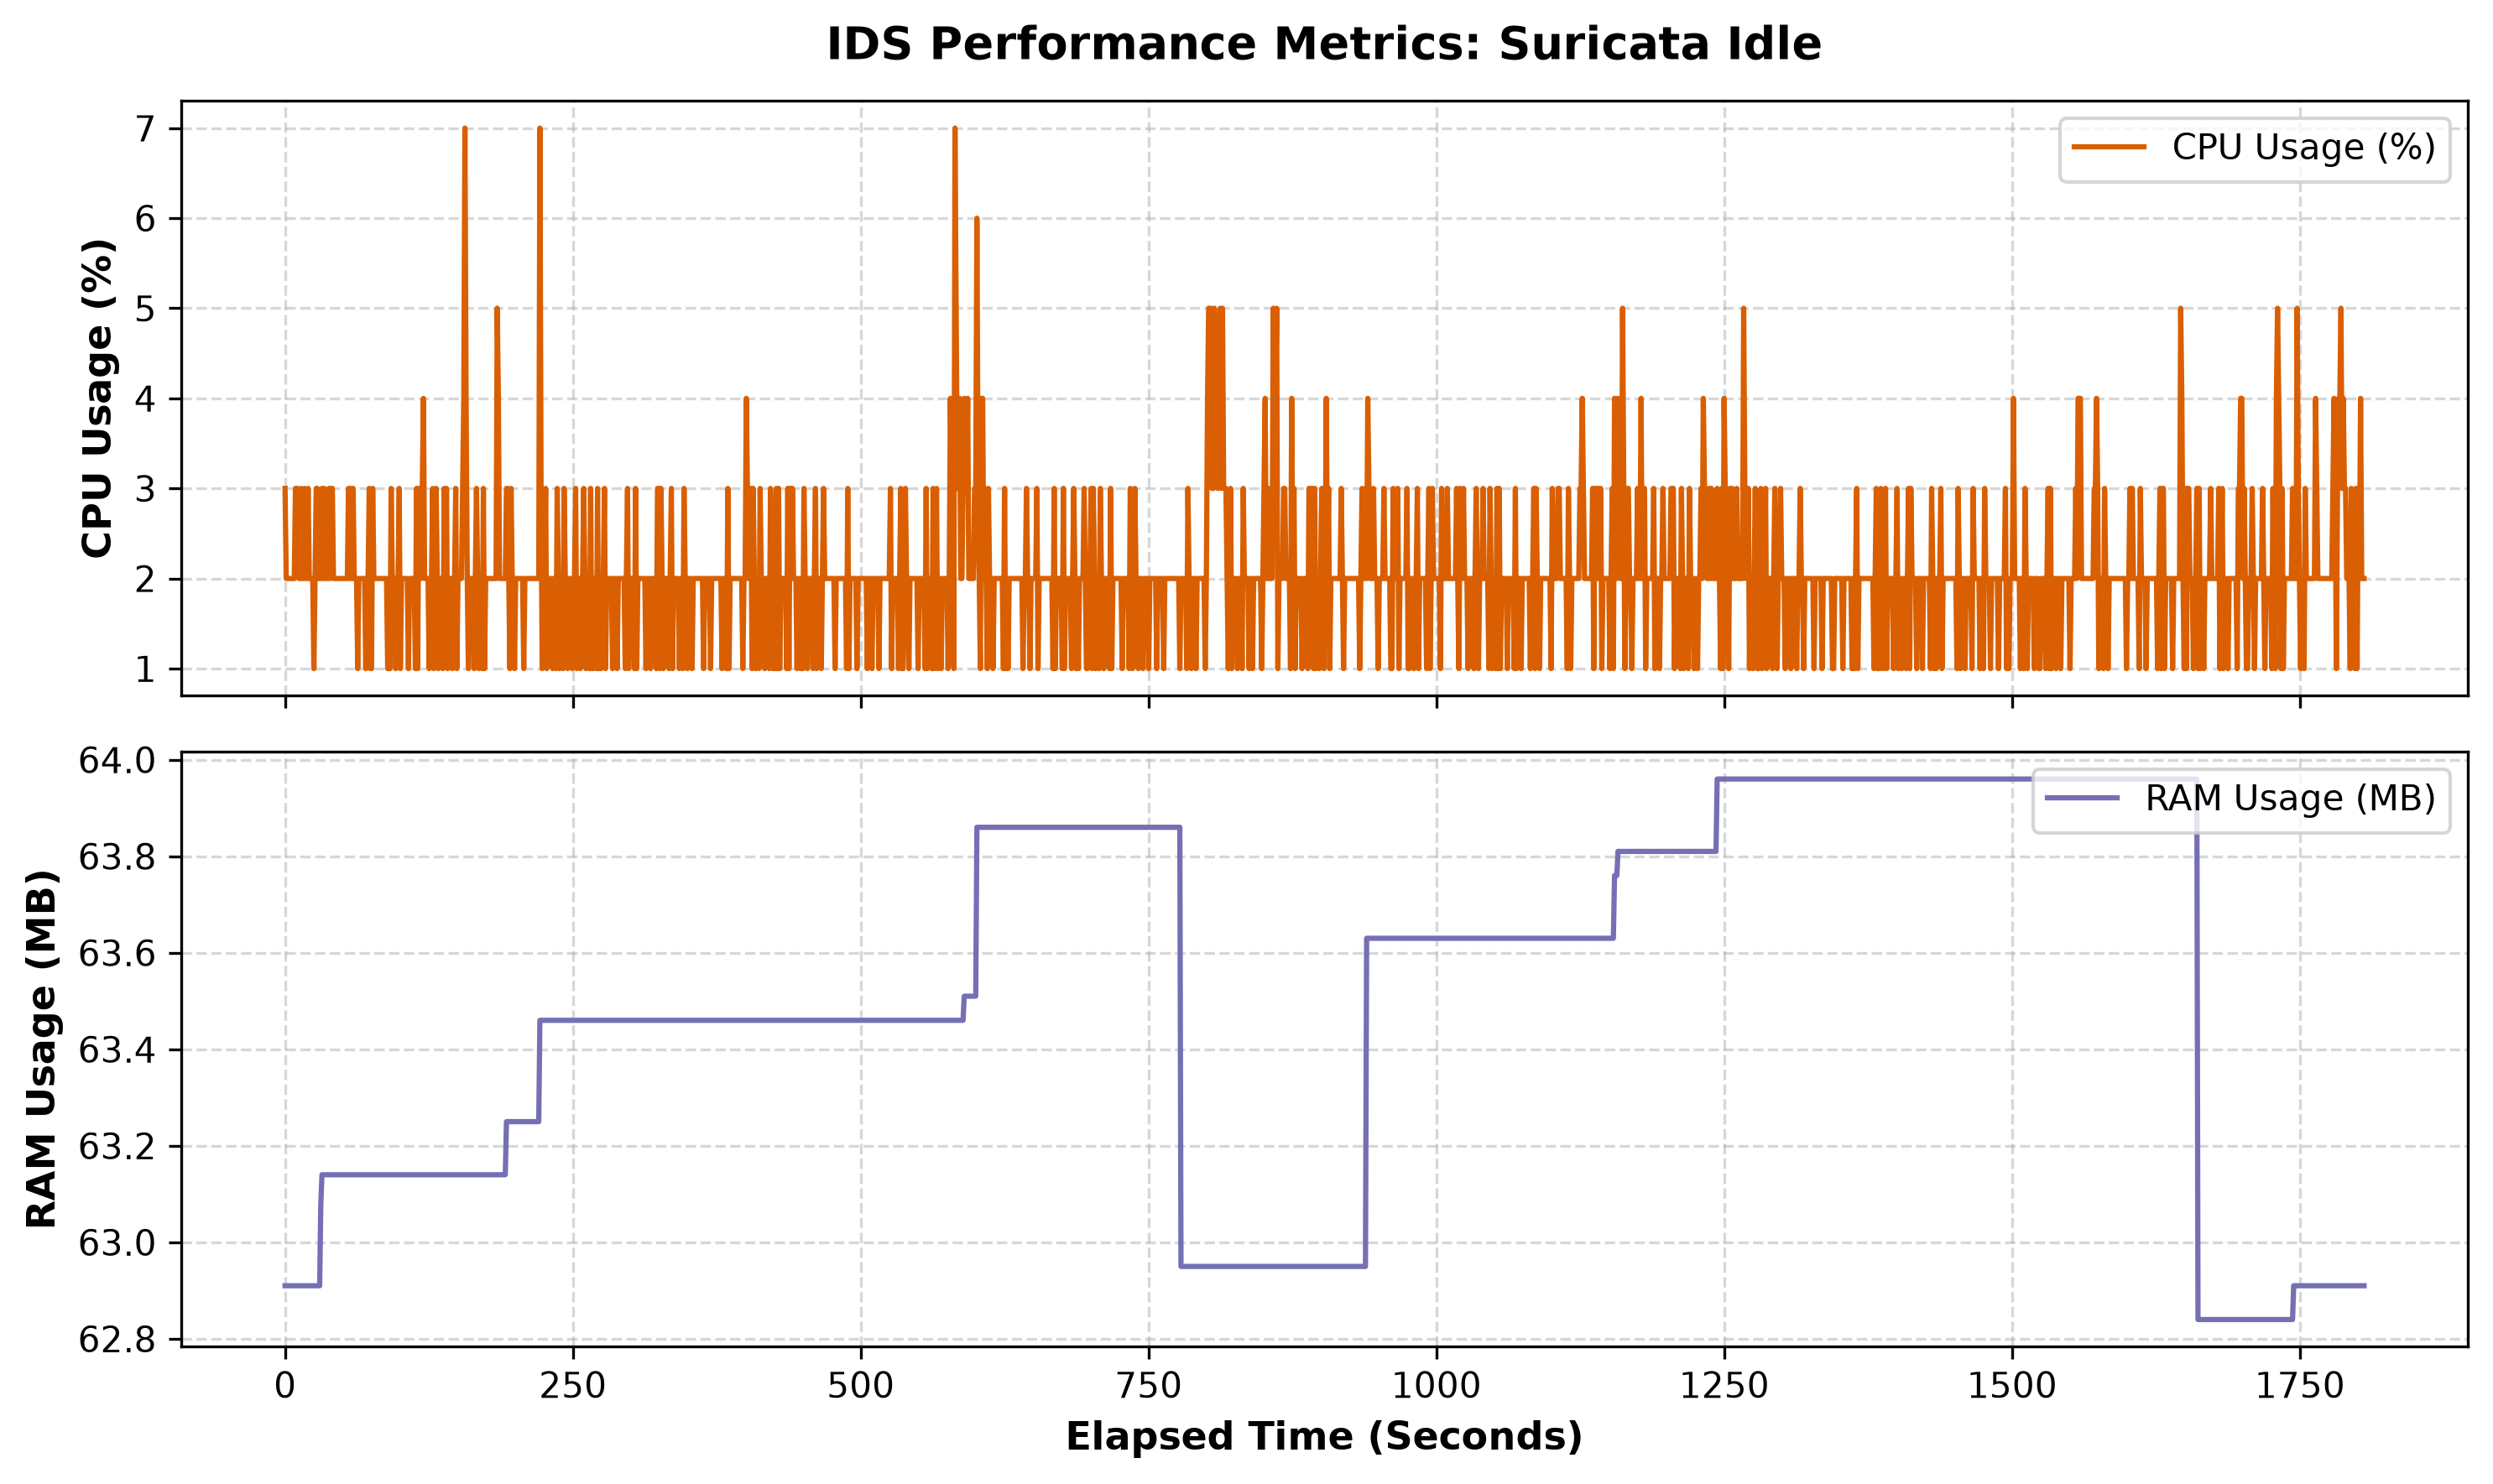
\includegraphics[width=0.7\textwidth]{../graphics/suricata_idle_plot.png}
    \caption{Systeemverbruik van Suricata tijdens de rusttoestand (idle-status).}
    \label{fig:suricata_idle}
\end{figure}

\begin{figure}[H]
    \centering
    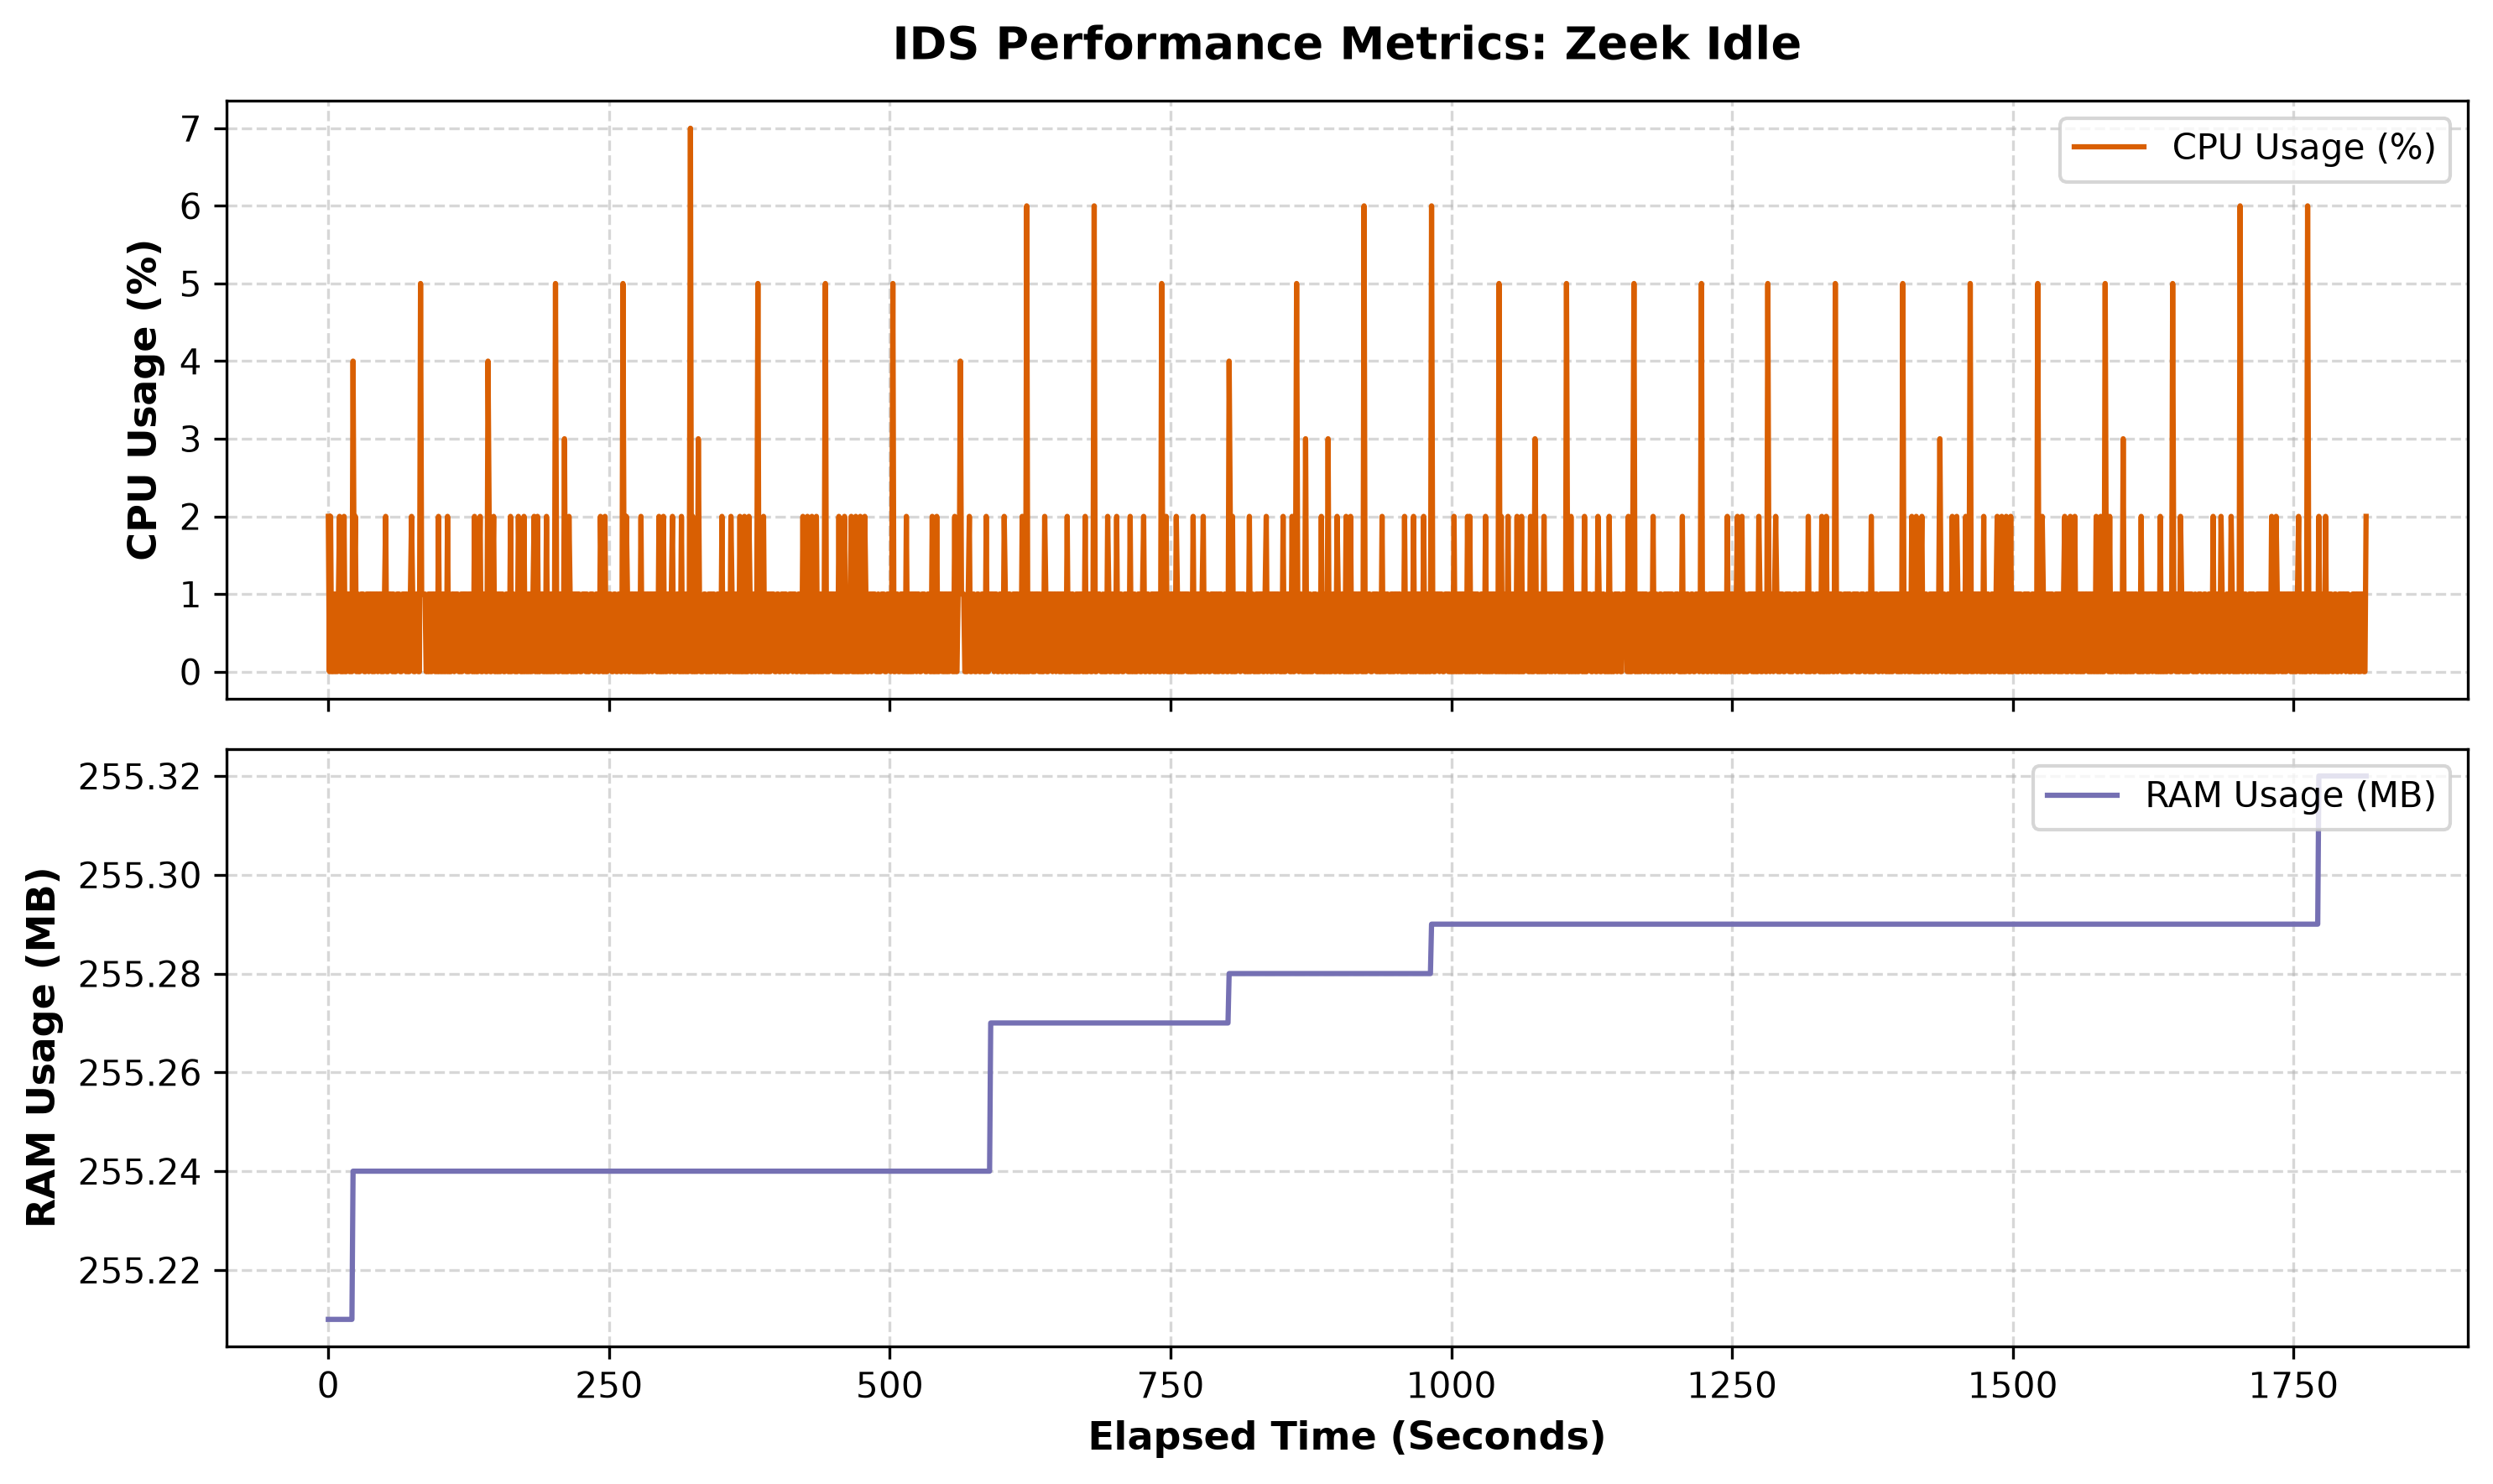
\includegraphics[width=0.7\textwidth]{../graphics/zeek_idle_plot.png}
    \caption{Systeemverbruik van Zeek tijdens de rusttoestand (idle-status).}
    \label{fig:zeek_idle}
\end{figure}


\begin{table}[H]
\centering
\renewcommand{\arraystretch}{1.2}
\begin{tabular}{|l|c|c|c|c|}
\hline
\textbf{IDS Engine} & \textbf{CPU (Gemiddeld)} & \textbf{CPU (Piek)} & \textbf{RAM (Gemiddeld)} & \textbf{RAM (Piek)} \\
\hline
\textbf{Suricata} & 2.05\% & 7.00\% & 63.52 MB & 63.96 MB \\
\hline
\textbf{Zeek} & 0.66\% & 7.00\% & 255.27 MB & 255.32 MB \\
\hline
\end{tabular}
\caption{Vergelijking van het CPU- en geheugenverbruik tijdens de rustfase (idle).}
\label{tab:idle_fase_vergelijking}
\end{table}

In deze fase bleek uit de metingen dat beide IDS-systemen pieken op circa 7\% CPU-gebruik, en dat Suricata gemiddeld 63,52 MB werkgeheugen in beslag neemt. Dat Zeek tijdens de rustfase meer werkgeheugen verbruikt dan Suricata, is grotendeels toe te schrijven aan de afwezigheid van een actieve regelset binnen de Suricata-configuratie.
Suricata is een signature-based IDS, wat betekent dat het geheugenverbruik sterk correleert met het aantal ingeladen detectieregels. Zonder een uitgebreide regelset is de basisvoetafdruk van de Suricata-engine relatief klein. Zeek functioneert daarentegen primair op basis van scripts en protocol-analyzers. Zelfs in een rustfase laadt Zeek standaard een aanzienlijke hoeveelheid basis-scripts en frameworks in het geheugen voor state management en netwerkanalyse, wat resulteert in een hogere initiële geheugenvoetafdruk.


\subsubsection{Operationele toestand (baseline)}
In tegenstelling tot de rustfase, waarin de systemen in een inactieve staat werkten, toont de operationele toestand een significant ander prestatieprofiel. Tijdens deze fase werd actief IoT-netwerkverkeer geïnjecteerd en werden beide systemen voorzien van hun volledige detectielogica: Suricata werd geconfigureerd met de uitgebreide Emerging Threats Open (ETO) regelset en de IoT regelset, terwijl Zeek werd alleen voorzien van IoT-detectiescripts. De resulterende meetgegevens leggen de fundamentele architecturale verschillen tussen beide IDS-engines bloot.

\begin{figure}[H]
    \centering
    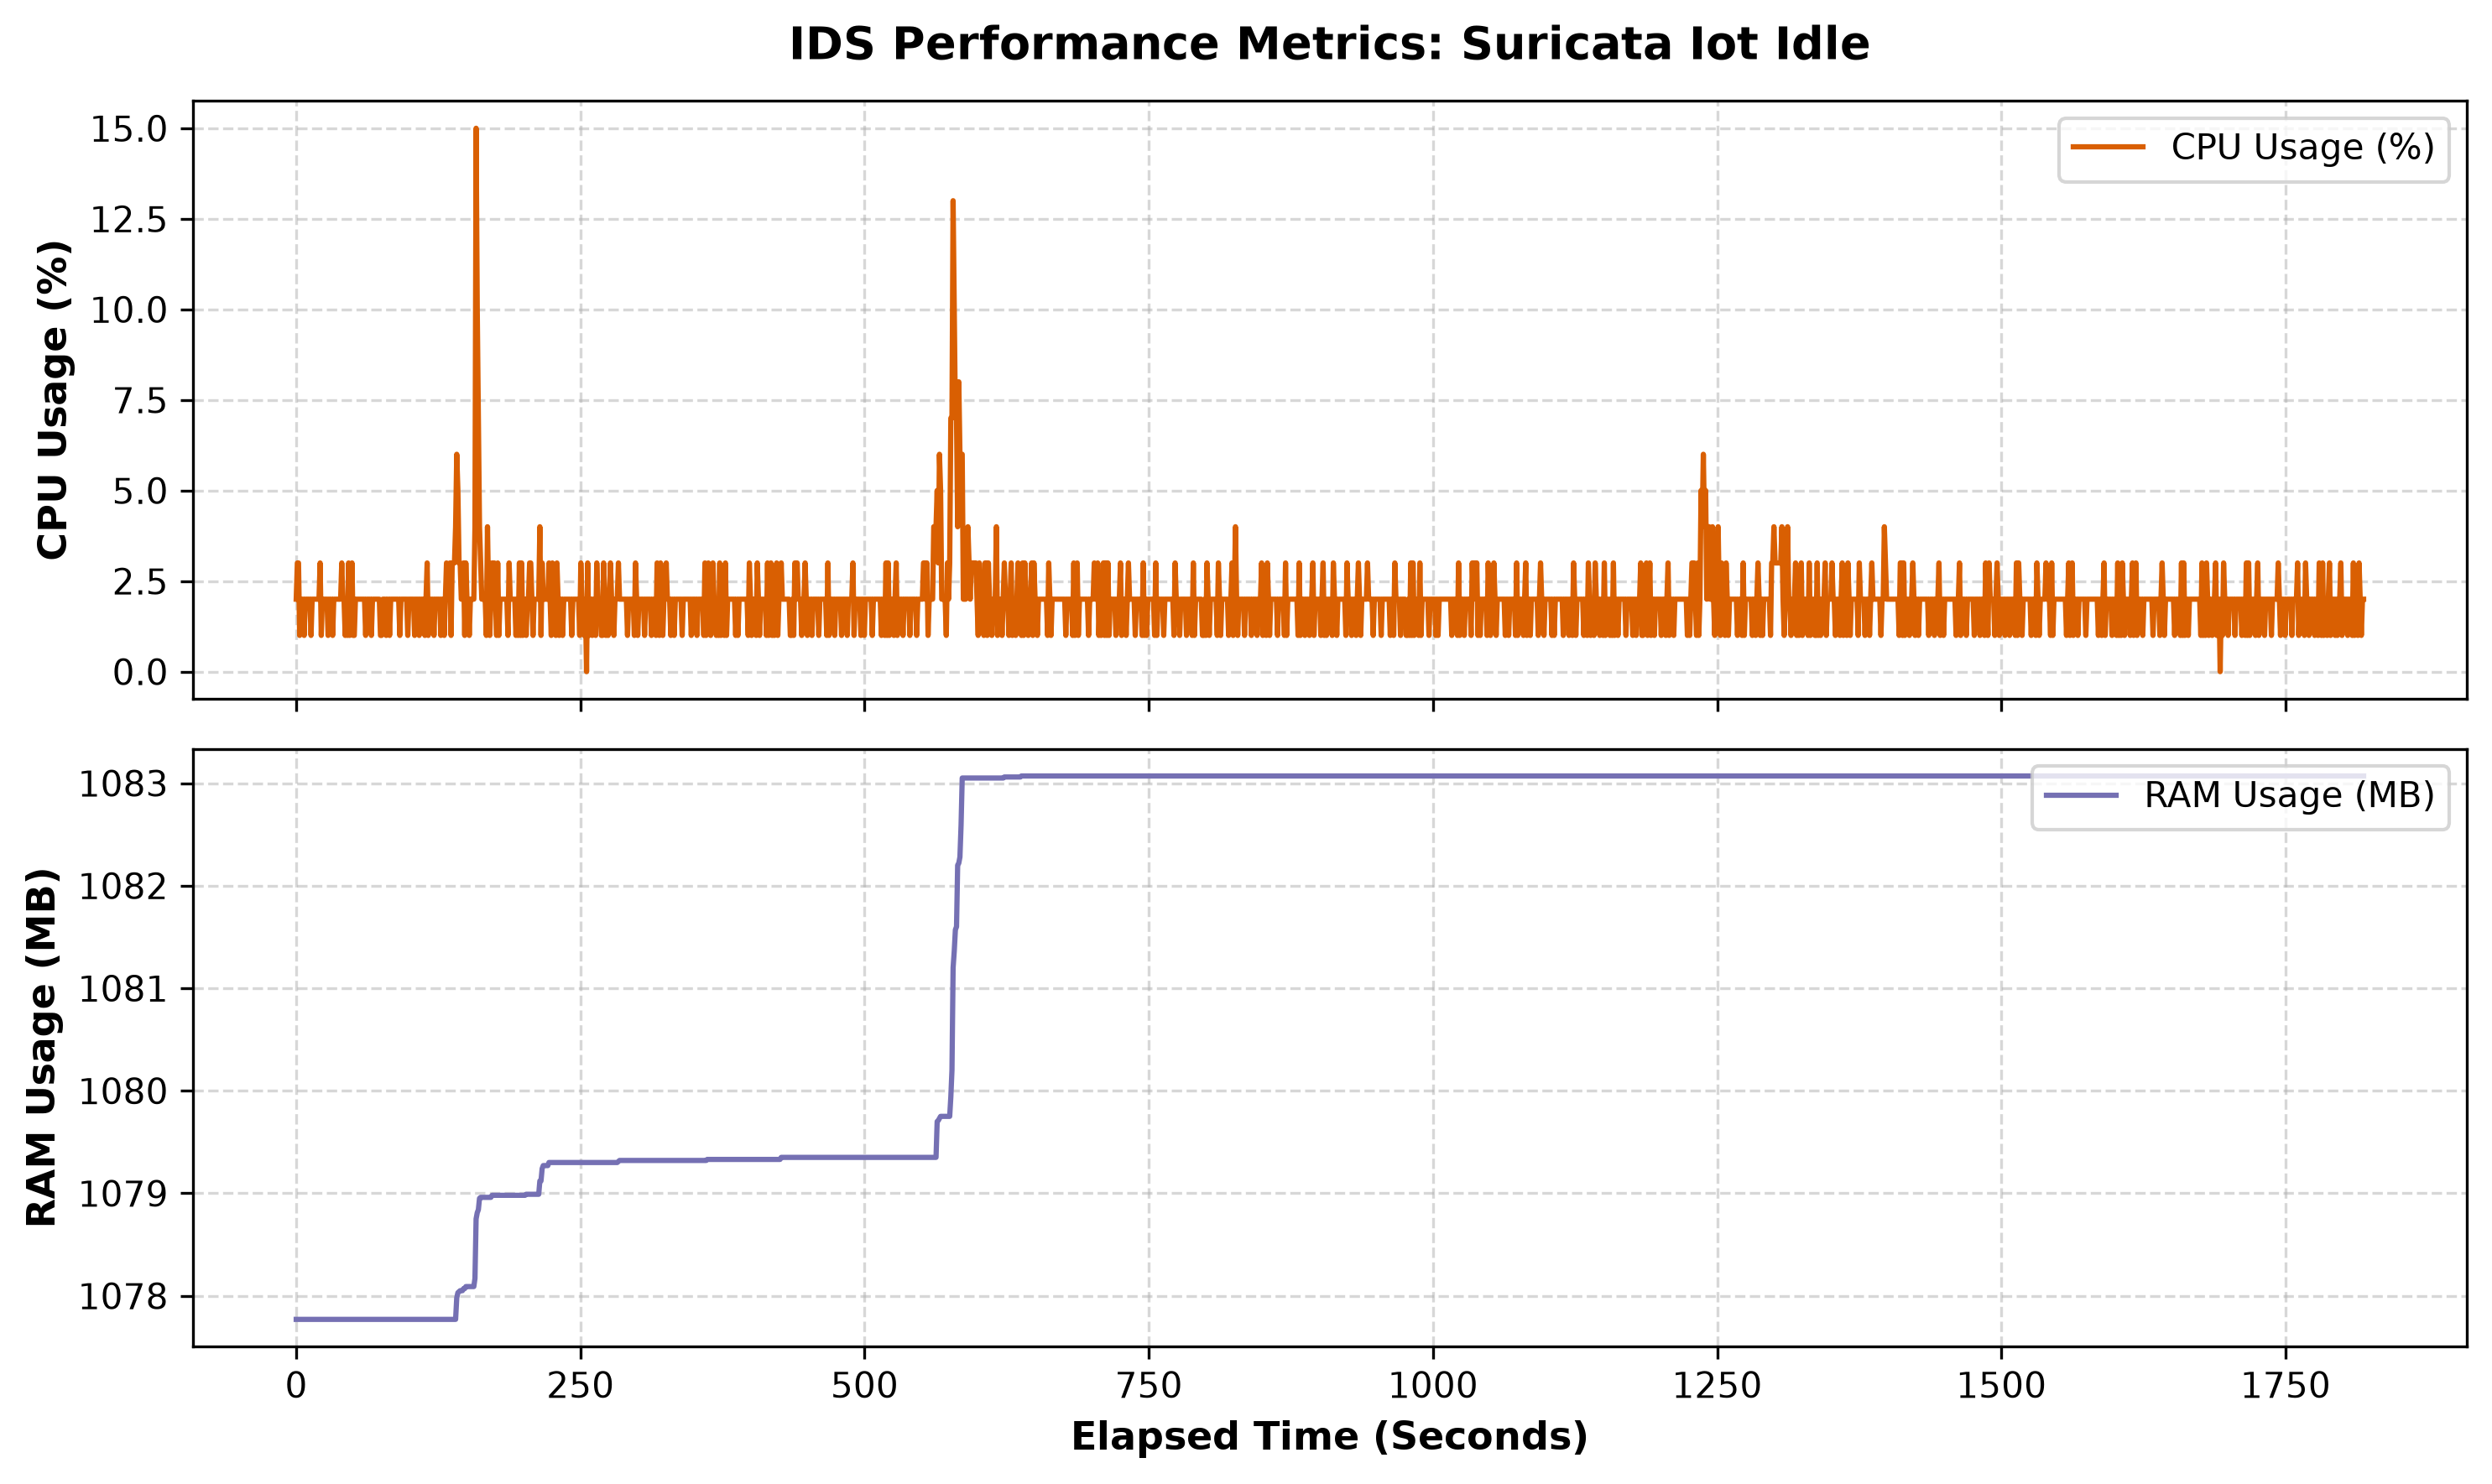
\includegraphics[width=0.7\textwidth]{../graphics/suricata_IoT_traffic_plot.png}
    \caption{Systeemverbruik van Suricata tijdens de operationele toestand (baseline-status).}
    \label{fig:suricata_baseline}
\end{figure}

\begin{figure}[H]
    \centering
    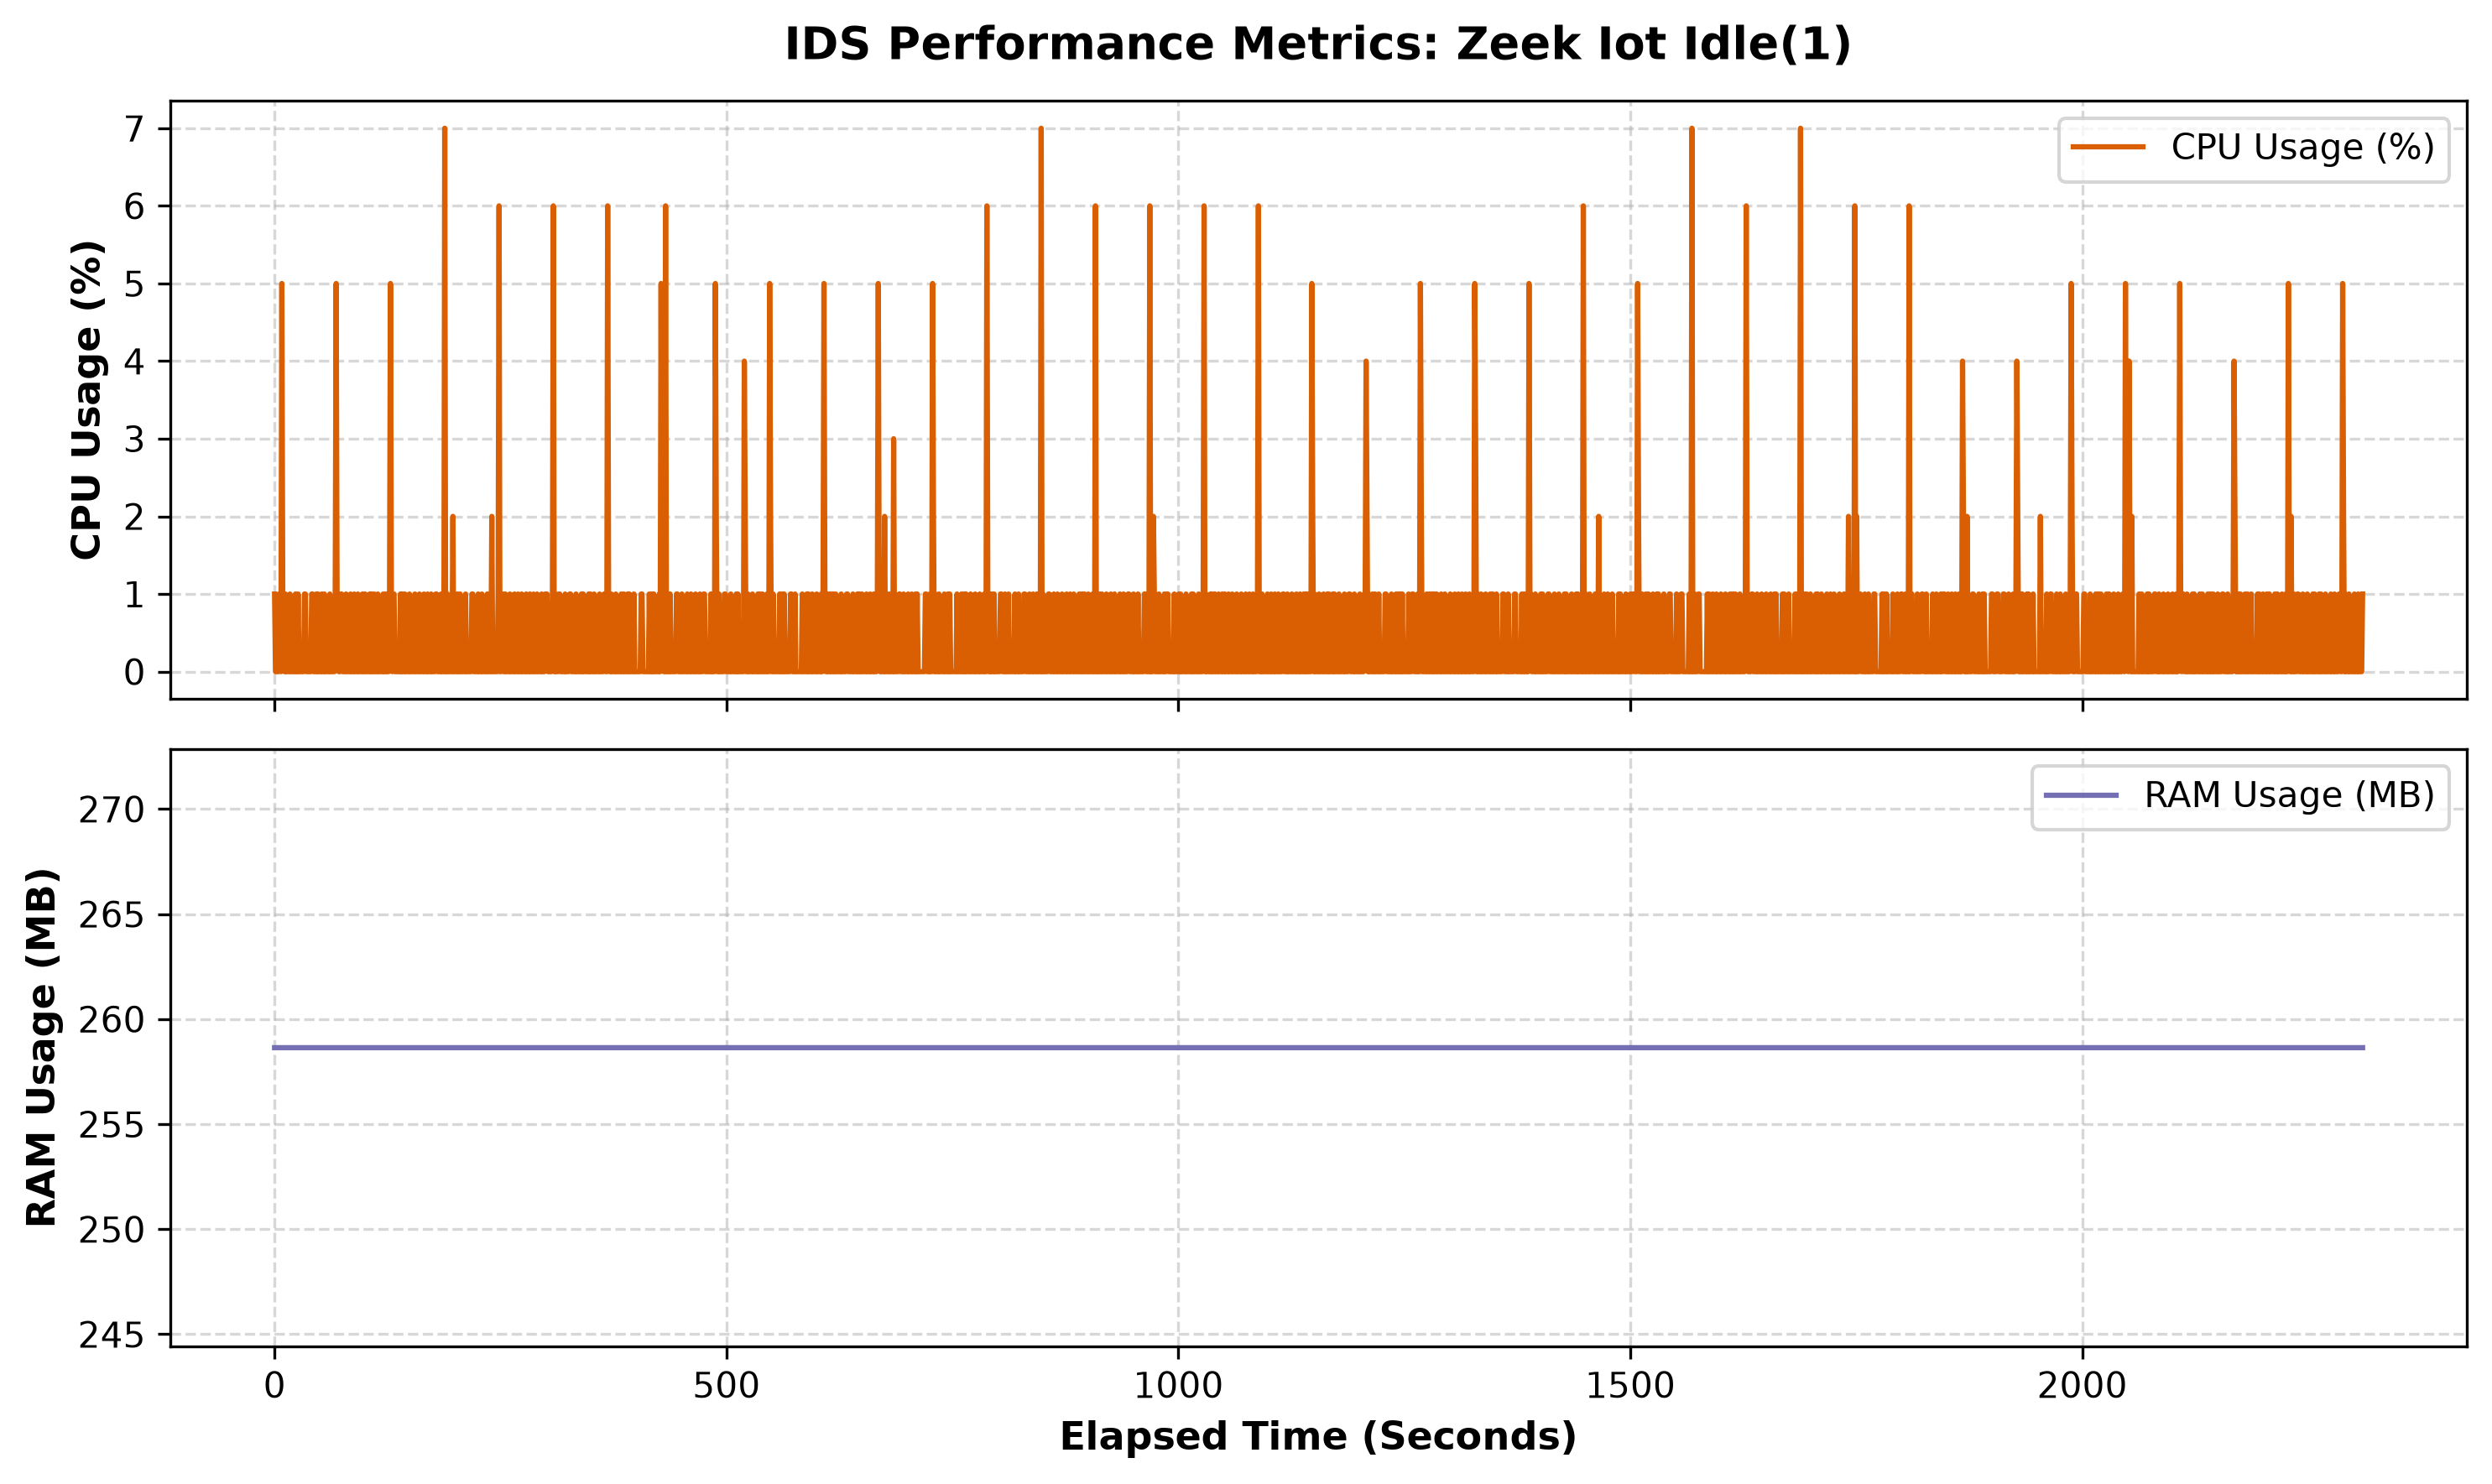
\includegraphics[width=0.7\textwidth]{../graphics/zeek_IoT_traffic_plot.png}
    \caption{Systeemverbruik van Zeek tijdens de operationele toestand (baseline-status).}
    \label{fig:zeek_baseline}
\end{figure}    

\begin{table}[H]
\centering
\renewcommand{\arraystretch}{1.2}
\begin{tabular}{|l|c|c|c|c|}
\hline
\textbf{IDS Engine} & \textbf{CPU (Gemiddeld)} & \textbf{CPU (Piek)} & \textbf{RAM (Gemiddeld)} & \textbf{RAM (Piek)} \\
\hline
\textbf{Suricata} & 1.98\% & 15.00\% & 1081.74 MB & 1083.07 MB \\
\hline
\textbf{Zeek} & 0.36\% & 7.00\% & 258.64 MB & 258.64 MB \\
\hline
\end{tabular}
\caption{Vergelijking van het CPU- en geheugenverbruik tijdens de operationele fase (actief IoT-verkeer).}
\label{tab:operationele_fase_vergelijking}
\end{table}

De meest opvallende verandering in deze fase is het werkgeheugengebruik van Suricata bij het inladen van de volledige regelset, terwijl Zeek een veel stabieler en lager geheugenprofiel vertoont. Dit is te verklaren door het feit dat Zeek functioneert als een dynamische protocol-analyzer met \textit{event-driven} scripts, in plaats van te vertrouwen op statische signatuurregels. Hierdoor is Zeek onder operationele belasting aanzienlijk efficiënter met het geheugen om.

Hoewel het gemiddelde CPU-gebruik bij beide IDS-systemen in deze fase is gedaald, valt op dat de CPU-piek van Suricata onder normale belasting is verdubbeld. Dit lagere gemiddelde kan worden verklaard doordat de systemen in een stabiele operatieve toestand zijn gekomen. Bovendien worden IoT-pakketten (zoals MQTT) verwerkt in kleine, snelle reeksen. Dit specifieke verwerkingsproces legt minder druk op de processor, wat resulteert in een lager gemiddeld CPU-percentage.



\subsubsection{Aanvalstoestand (stress-test)}

Nadat er een referentiepunt voor normaal netwerkverkeer is vastgesteld, kan worden onderzocht hoe de NIDS-systemen presteren tijdens een cyberaanval. In deze fase wordt de IoT-omgeving actief blootgesteld aan netwerkaanvallen. Het primaire doel hiervan is om te analyseren hoe beide detectiesystemen reageren wanneer de infrastructuur onder druk staat, waarbij elke aanval nauwkeurig wordt gelogd.

\begin{figure}[H]
    \centering
    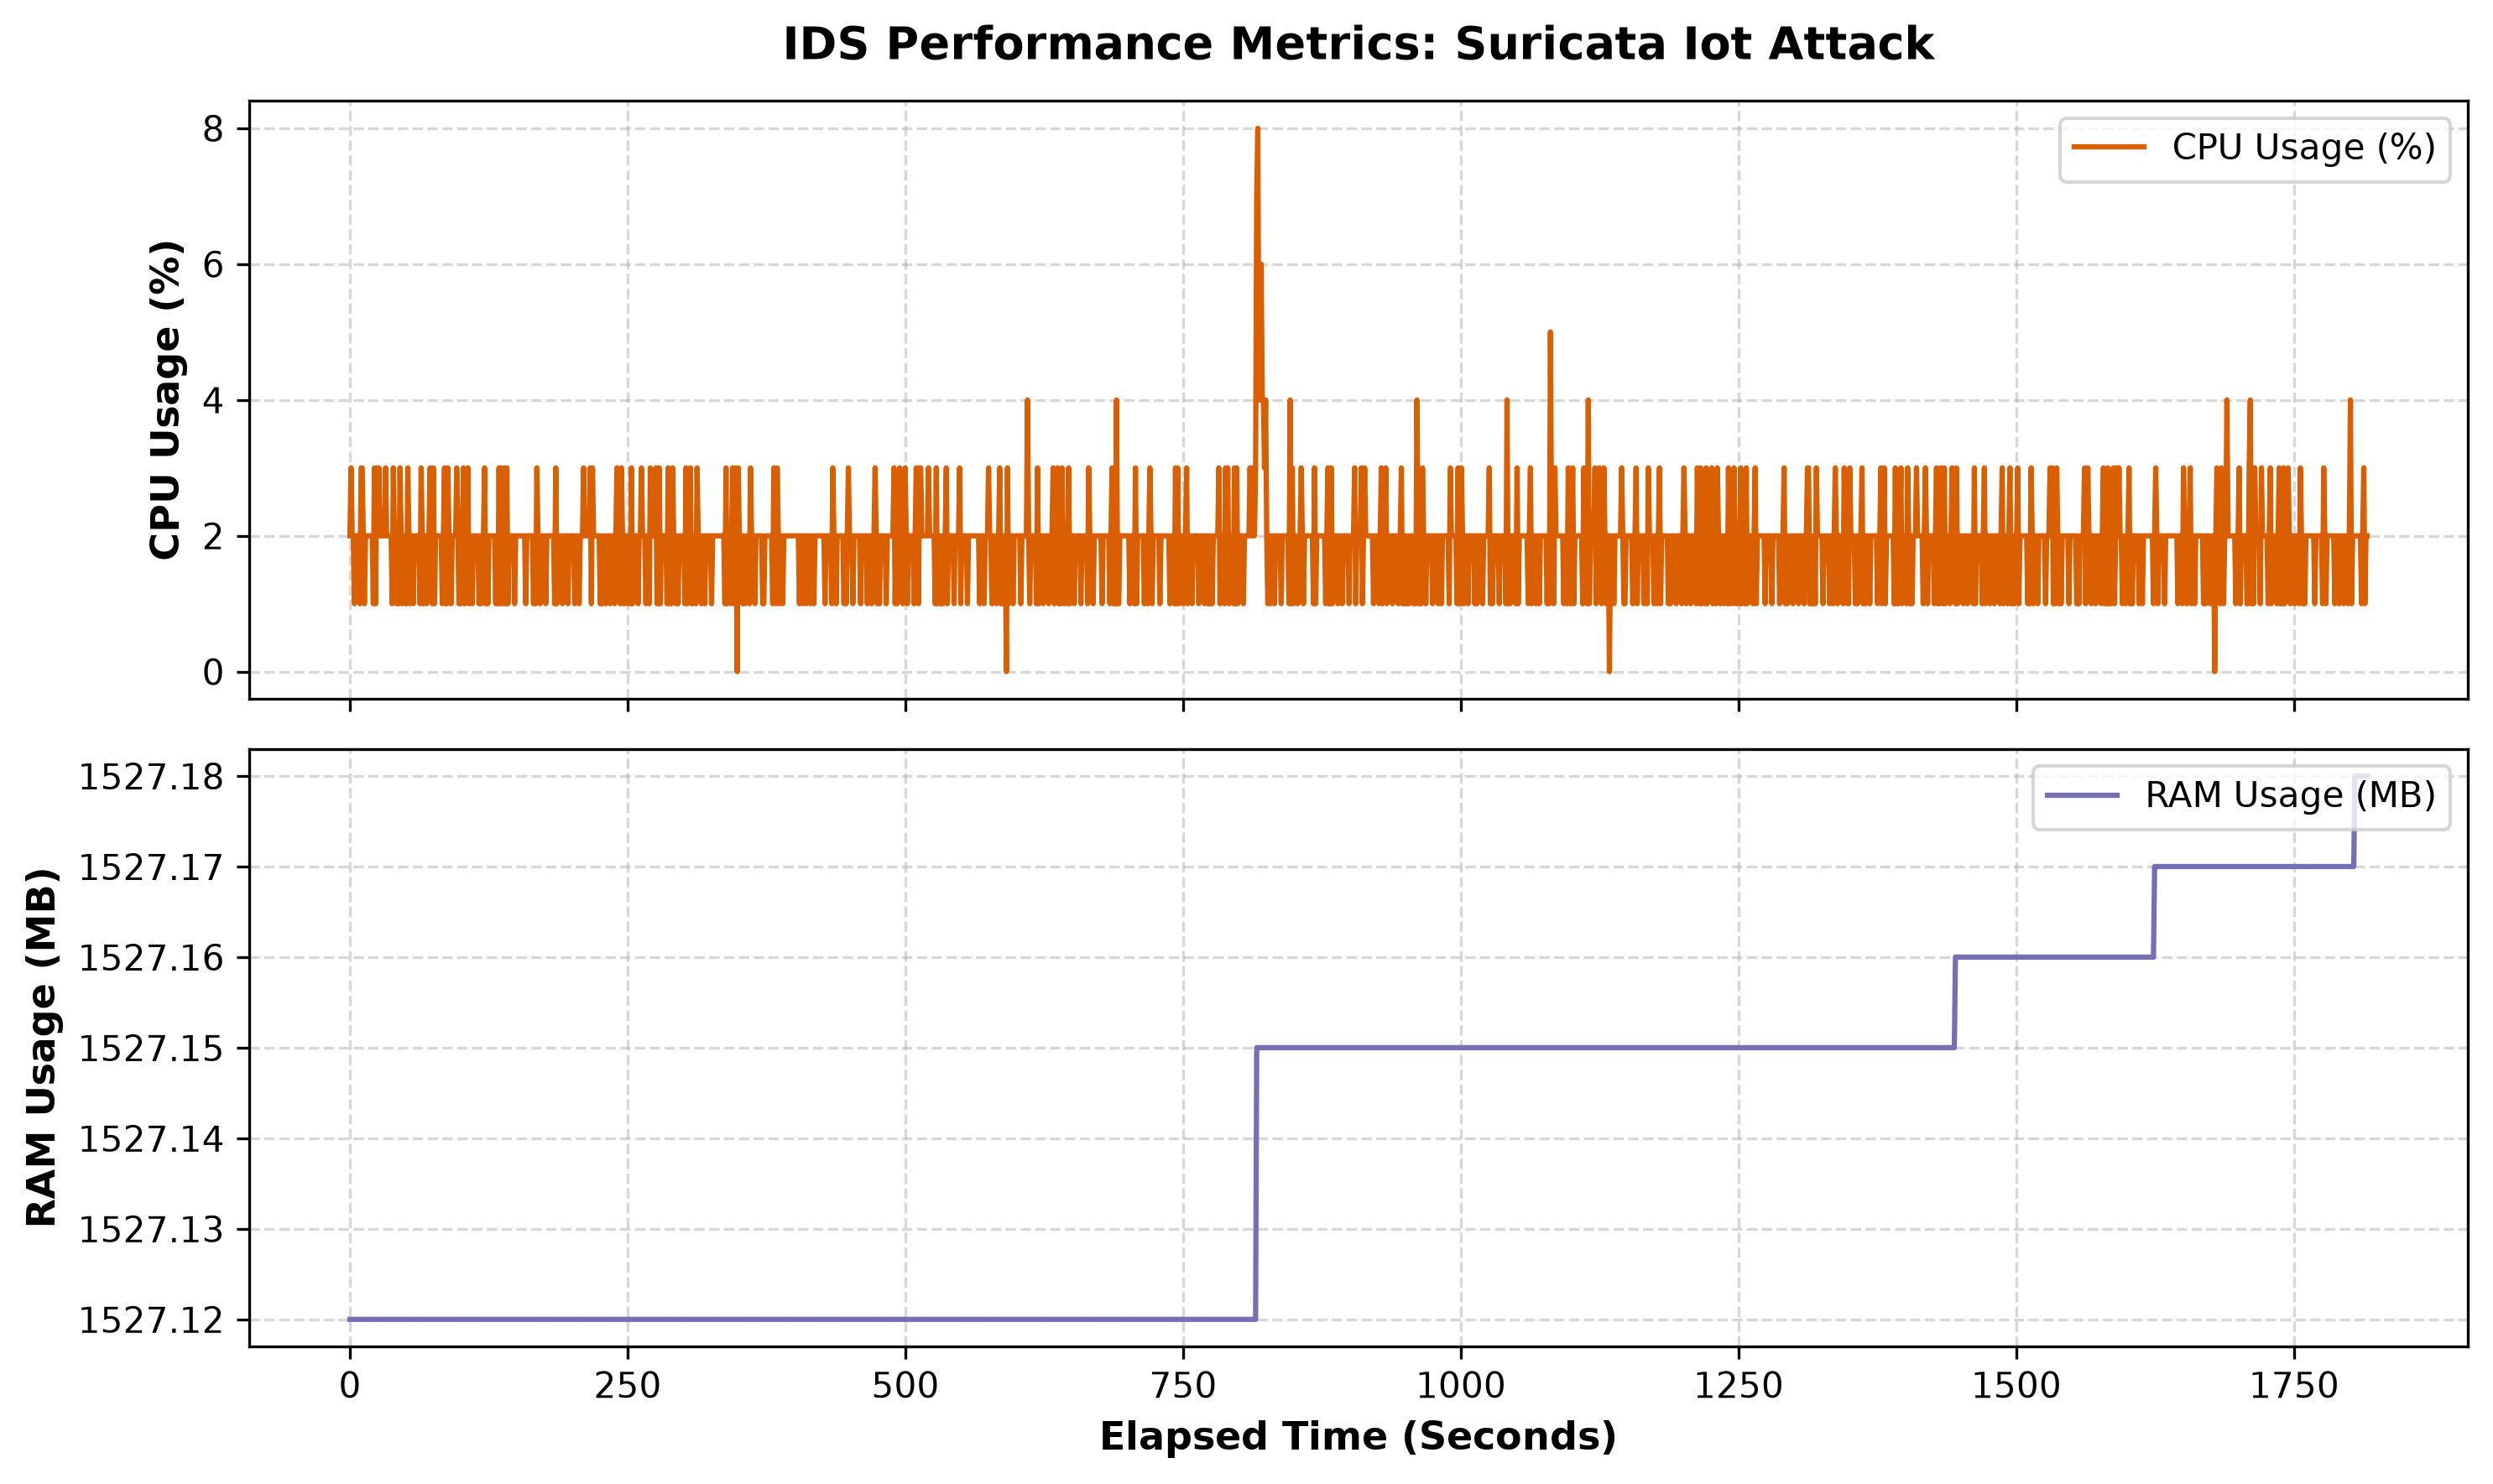
\includegraphics[width=0.7\textwidth]{../graphics/suricata_IoT_attack_plot.png}
    \caption{Systeemverbruik van Suricata tijdens de aanvalstoestand (stress-test).}
    \label{fig:suricata_attack}
\end{figure}

\begin{figure}[H]
    \centering
    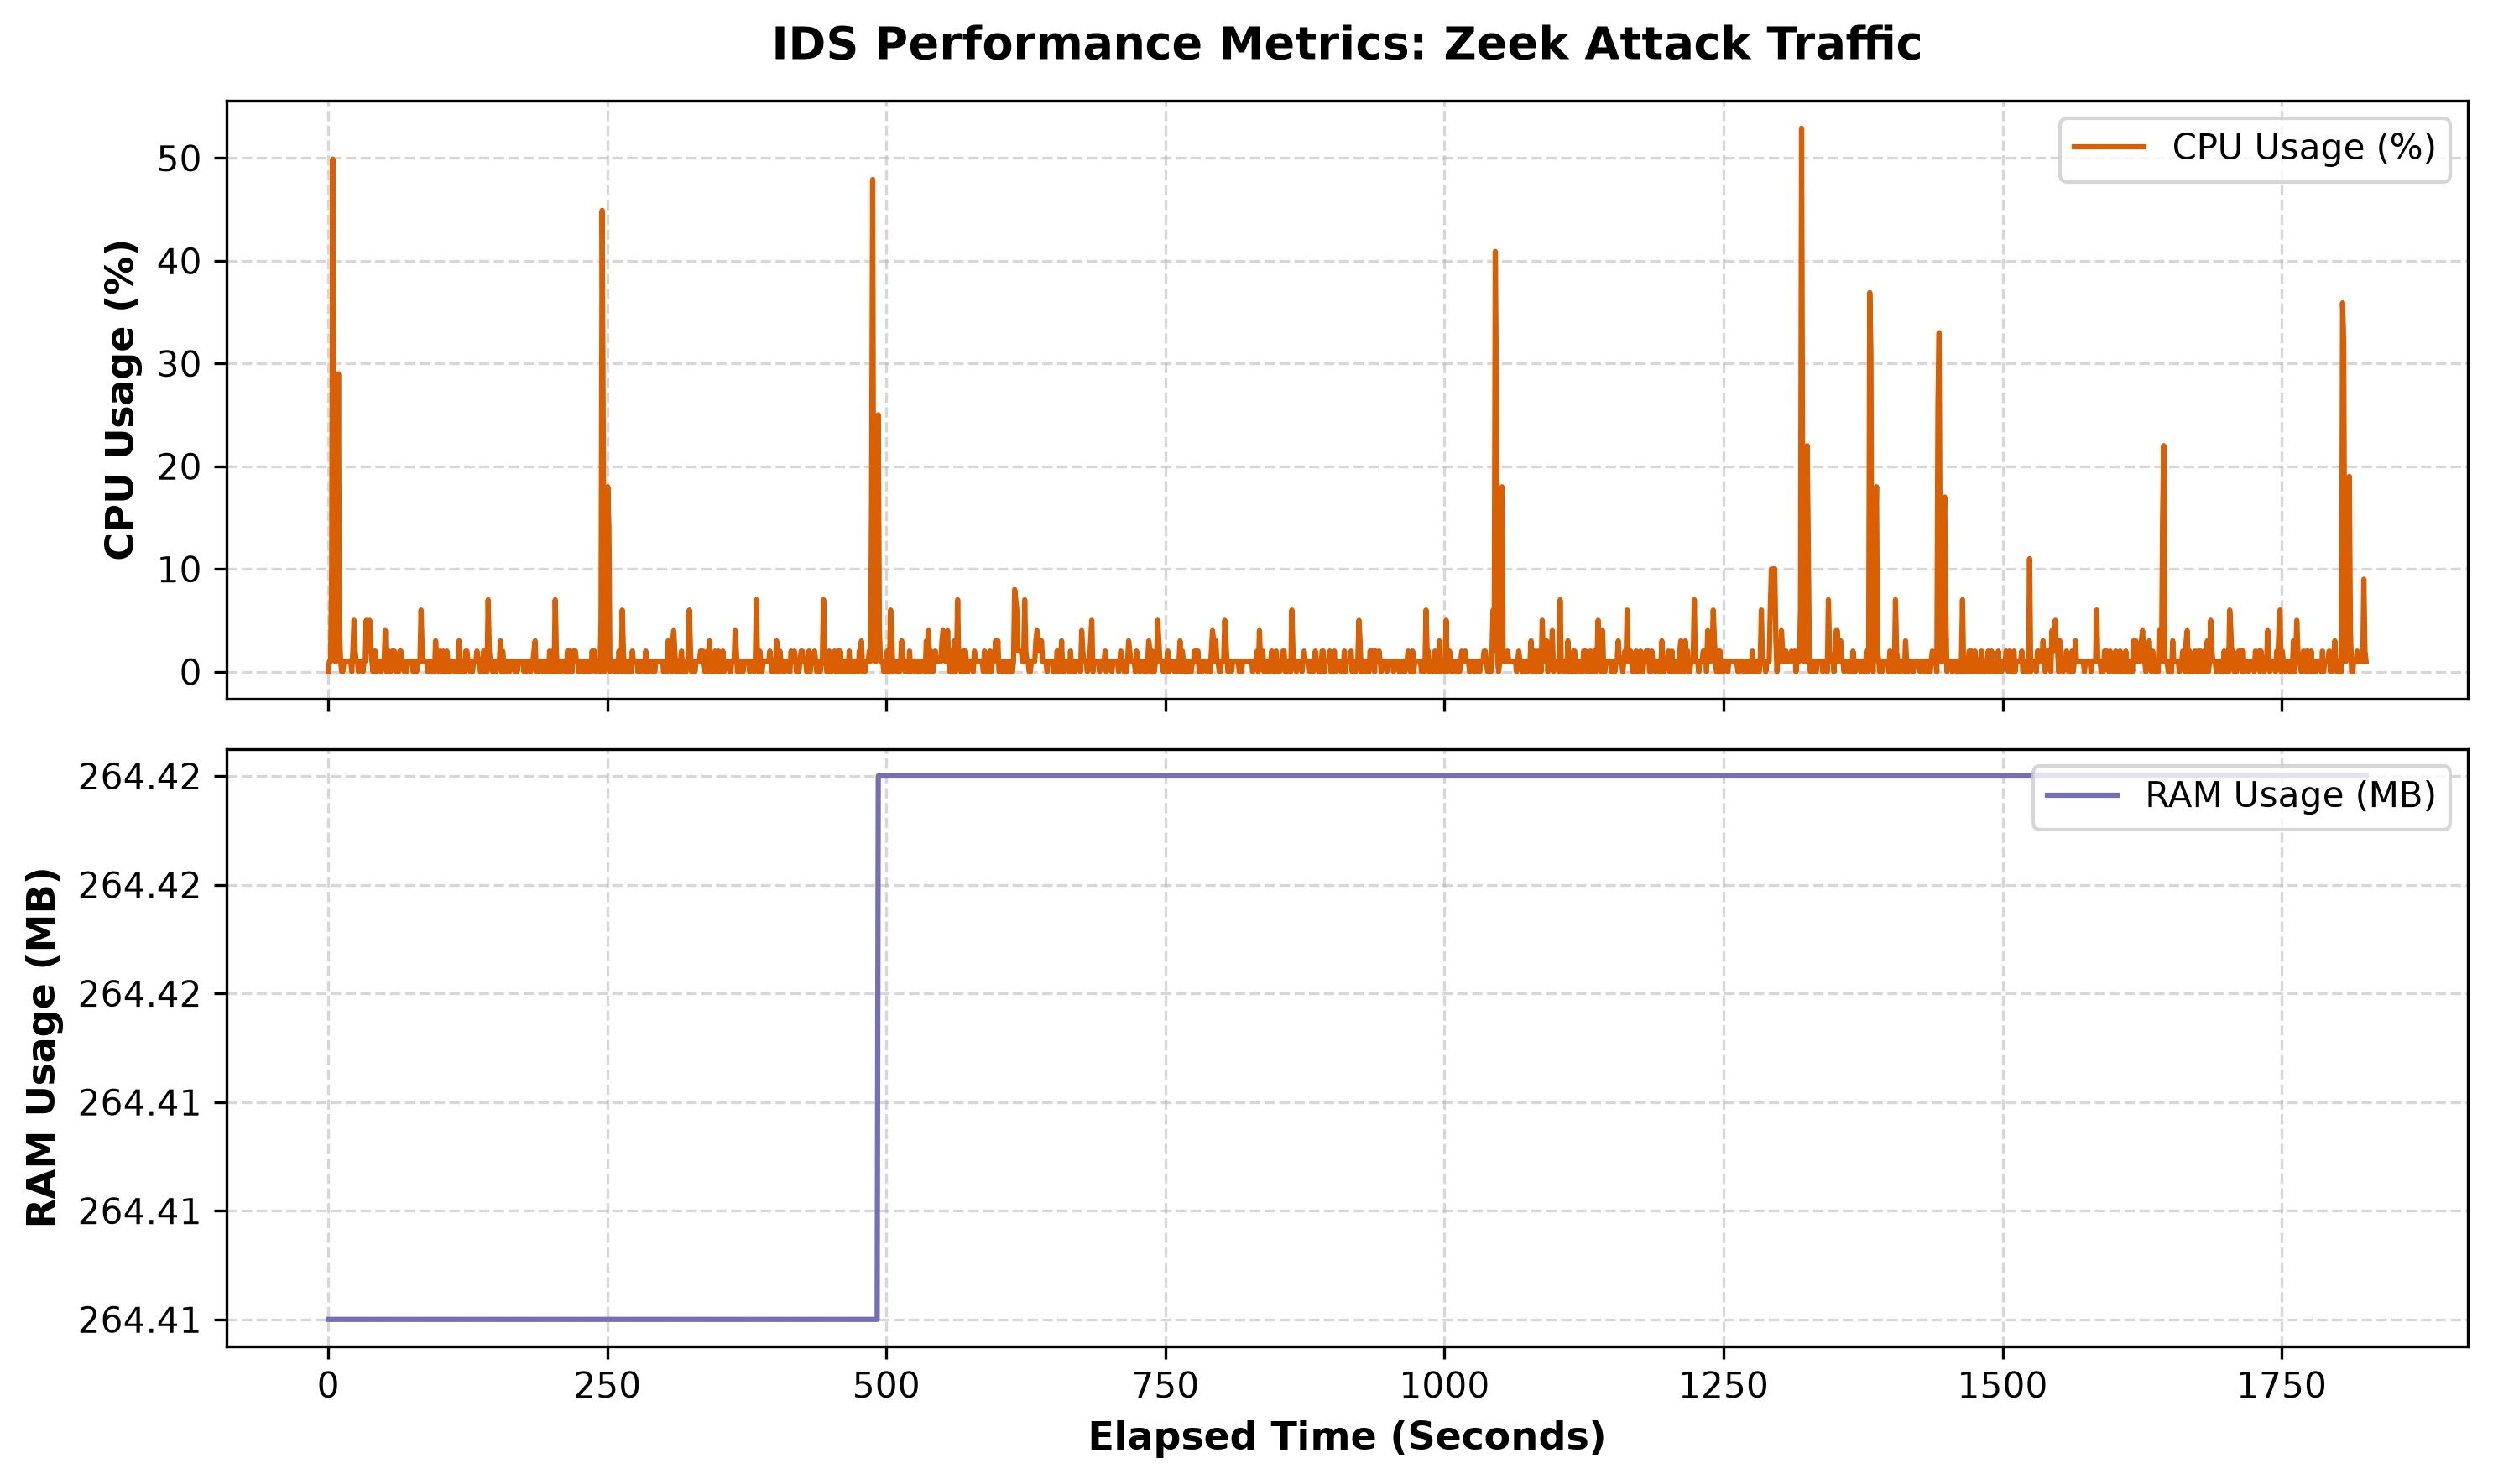
\includegraphics[width=0.7\textwidth]{../graphics/zeek_attack_traffic_plot.png}
    \caption{Systeemverbruik van Zeek tijdens de aanvalstoestand (stress-test).}
    \label{fig:zeek_attack}
\end{figure}

\begin{table}[H]
\centering
\renewcommand{\arraystretch}{1.2}
\begin{tabular}{|l|c|c|c|c|}
\hline
\textbf{IDS Engine} & \textbf{CPU (Gemiddeld)} & \textbf{CPU (Piek)} & \textbf{RAM (Gemiddeld)} & \textbf{RAM (Piek)} \\
\hline
\textbf{Suricata} & 1.89\% & 8.00\% & 1527.14 MB & 1527.18 MB \\
\hline
\textbf{Zeek} & 1.55\% & 52.90\% & 264.42 MB & 264.42 MB \\
\hline
\end{tabular}
\caption{Vergelijking van het CPU- en geheugenverbruik tijdens de aanvalstoestand.}
\label{tab:aanvalstoestand_vergelijking}
\end{table}


Bij de analyse van de aanvalsscenario's vallen direct enkele opmerkelijke patronen in de grafieken op. Voor Suricata zien we dat het gemiddelde RAM-verbruik stijgt naar 1527 MB, wat neerkomt op een significante toename van 41,17\% ten opzichte van de normale operationele fase. Het geheugenverbruik van Zeek blijft daarentegen stabiel in vergelijking met de voorgaande fases. Wat we bij Zeek echter wel waarnemen, is dat het CPU-gebruik tijdens het uitvoeren van een DoS-aanval een enorme piek bereikt van 52,90\%.